\documentclass[twoside]{protokoll}
\usepackage{graphicx}
\usepackage{tabularx}
\usepackage{booktabs}
\usepackage{float} 
\praktikum{I}
\usepackage{subfig}
\usepackage{amsmath}

\versuchsgebiet{(Mechanik)}


\teilnehmer{Maximilian Carlos Menke, 434170}
\teilnehmer{Andrea Roth, 428396}
\gruppe{A3}

\begin{document}
 
\section{1M1 Messung der Erdbeschleunigung mit dem Pendel}
 
\begin{aufgabe}{Grundlagen}
  Knappe Beschreibung der theoretischen Grundlagen, Angabe der
  benötigten Formel(n), ohne Herleitung. Definition der verwendeten
  Formelzeichen.
\end{aufgabe}

\section{Grundlagen}

Ein Pendel kann als physikalisches Pendel beschrieben werden.
Dabei wirkt auf das Pendel eine Kraft von $F_g = m_S \cdot g$, wobei $g$ die zu bestimmende Erdbeschleunigung ist und $m_S$ die Schwere Masse des Pendels.
Beim Schwingen, befindet sich das Pendel oftmals nicht in der Ruhelage, sondern ist in einer Auslenkung $\varphi$ vom Gleichgewichtszustand entfernt.
Dann wirkt ein rückstellendes Drehmoment $ M = l \cdot F_r$ (mit $l$ als Länge von der Rotationsachse zum Schwerpunkt).
Da unser Pendel Träge ist, entsteht eine Schwingung: 
\begin{equation}
    J \cdot \ddot{\varphi} = -m \cdot g \cdot l^2 \cdot \sin(\varphi)
\end{equation}
Dabei verwenden wir im Folgenden die Kleinwinkel Näherung $\sin(\varphi) \approx \varphi$.
Diese gilt für Auslenkungen von weniger als $5$°. Damit lässt sich die Bewegungsgleichung vereinfachen:
\begin{equation}
    J \cdot \ddot{\varphi} \approx -m \cdot g \cdot l^2 \cdot \varphi
\end{equation}
Das Trägheitsmoment ist dabei wie folgt definiert:
\begin{equation}
    J =  m_T \cdot l^2
\end{equation}
Hierbei ist $m_T$ die Träge Masse des Pendels. Dies ist nach dem Einsteinnischen Äquivalenzprinzip aber gleich der schweren Masse, und somit $m_T = m$.
Aufgelöst nach $\ddot{\varphi}$ ergibt sich ( mit $\omega = 2 \pi f = \frac{2 \pi}{T}$ als Winkelgeschwindigkeit der Schwingung):
\begin{equation}
    \ddot{\varphi} \approx -\frac{g}{l} \cdot \varphi = - \omega^2 \cdot \varphi
\end{equation}
Aus dieser DGL lässt sich $\varphi(t)$ bestimmen, zu:
\begin{equation}
    \varphi(t) = \varphi_{max} \cdot \cos(\omega \cdot t)
\end{equation}
Daraus ergibt sich (mit $T$ als dauer einer Schwingungsperiode):
\begin{equation}
    \omega^2 = \frac{m \cdot g \cdot l_s}{J}
\end{equation}
\begin{equation}
    \Rightarrow T = \frac{1}{g} 4 \cdot \pi^2 \cdot \frac{J}{m l_s}
\end{equation}
Dabei kann man $\omega$ als Quotient von rückstellendes Drehmoment und Trägheitsmoment beschreiben.
Hier sind alle Größen mit einem einem G versehen sind dem Gewicht zugehörig. Die mit einem $_st$ versehenen Größen gehören nur zur Stange.
\begin{equation}
    \omega_{st}^2 = \frac{M_{st}}{J_{st}}
\end{equation}
\begin{equation}
    \omega_{G}^2 = \frac{M_G}{J_G}
\end{equation}
Wenn man die Position des Gewichtes so einstellt, dass die Schwingung der Stange die gleiche Periodendauer hat wie die Schwingung des Gewichtes, dann gilt:
\begin{equation}
    \omega_{st}^2 = \omega_{G}^2
\end{equation}
\begin{equation}
    \omega^2 = \frac{M_{st}}{J_{st}} = \frac{M_G}{J_G}
\end{equation}
Das bedeutet das wir das Pendel mit Gewicht so behandeln können, als würde nur der Pendelkörper schwingen. 
Es macht also kein Unterschied, ob wir die Stange weg lassen oder den Pendelkörper in unseren Berechnungen.
Das Trägheitsmoment des Gewichtes (der 1. Summand) und das zusätzliche Trägheitsmoment welches durch die Verschiebung der Rotationsachse mit dem Satz von Steiner hinzukommt:
\begin{equation}
    J_G = \frac{1}{2} m_G \cdot r_G^2 + m_G \cdot l_G^2
\end{equation}
Hier ist $r_G$ der Radius des Gewichtes und $l_G$ der Abstand vom Gewicht zur Rotationsachse.
Wenn man das Drehmoment und das Trägheitsmoment jetzt explizit ausdrückt, dann erhält man:
\begin{equation}
    \omega^2 = \frac{m_G \cdot g \cdot l_G}{\frac{1}{2} m_G \cdot r_G^2 + m_G \cdot l_G^2}
\end{equation}
Nach g Aufgelöst ergibt sich:
\begin{equation}
    g = \omega^2 \cdot l_G \left( 1 + \frac{r_G^2}{2 \cdot l_G^2} \right)
    \label{eq:pendel_g}
\end{equation}


Die Auslenkung des Winkels messen wir dabei mit der Hall-Sonde.
Das Magnetfeld kann dabei so orientiert werden, dass es vertikal steht.
Die Hall-Spannung wird dabei von der Hall-Konstante und  der Dicke des stromdurchflossenen Plättchens beeinflusst.
Hinzu kommt noch das Kreuzprodukt von Magnetfeld und Stromdurchfluss. Da sowohl das Magnetfeld als auch der Stromdurchfluss konstant sind, hängt das Kreuzprodukt nur von vom Sinus des Winkels der beiden ab.
Da wir nur kleine Winkel betrachten, kann man in guter Näherung annehmen, das $\sin(\varphi) \approx \varphi$ ist.
Folglich ist die Hall-Spannung nur proportional zur Auslenkung des Winkels, da alle anderen Größen konstant sind.



\begin{aufgabe}{Versuchsaufbau und Versuchsdurchführung}
  Beschreibung des Versuchsaufbaus einschließlich beschrifteter Skizze
  oder Foto. Beschreibung der Versuchsdurchführung: Handgriffe an der
  Apparatur, verwendete Messwerterfassungseinstellungen, Messbereiche,
  Triggerbedingungen, etc.
\end{aufgabe}

\section{Aufbau und Durchführung}
Kurz zusammengefasst besteht der Versuchsaufbau aus einem Stabilen dreieckigen Stativ, an welchem ein Winkelaufnehmer befestigt wird.
An diesen Winkelaufnehmer Wird ein Pendel gehangen, welches aus einem U-Profil, mit zwei Metallnadeln als Aufhängung, einer flachen Pendelstange, und einem Pendelkörper besteht.\\
\subsection{Aufbau}
\begin{figure}[H]
    \centering
    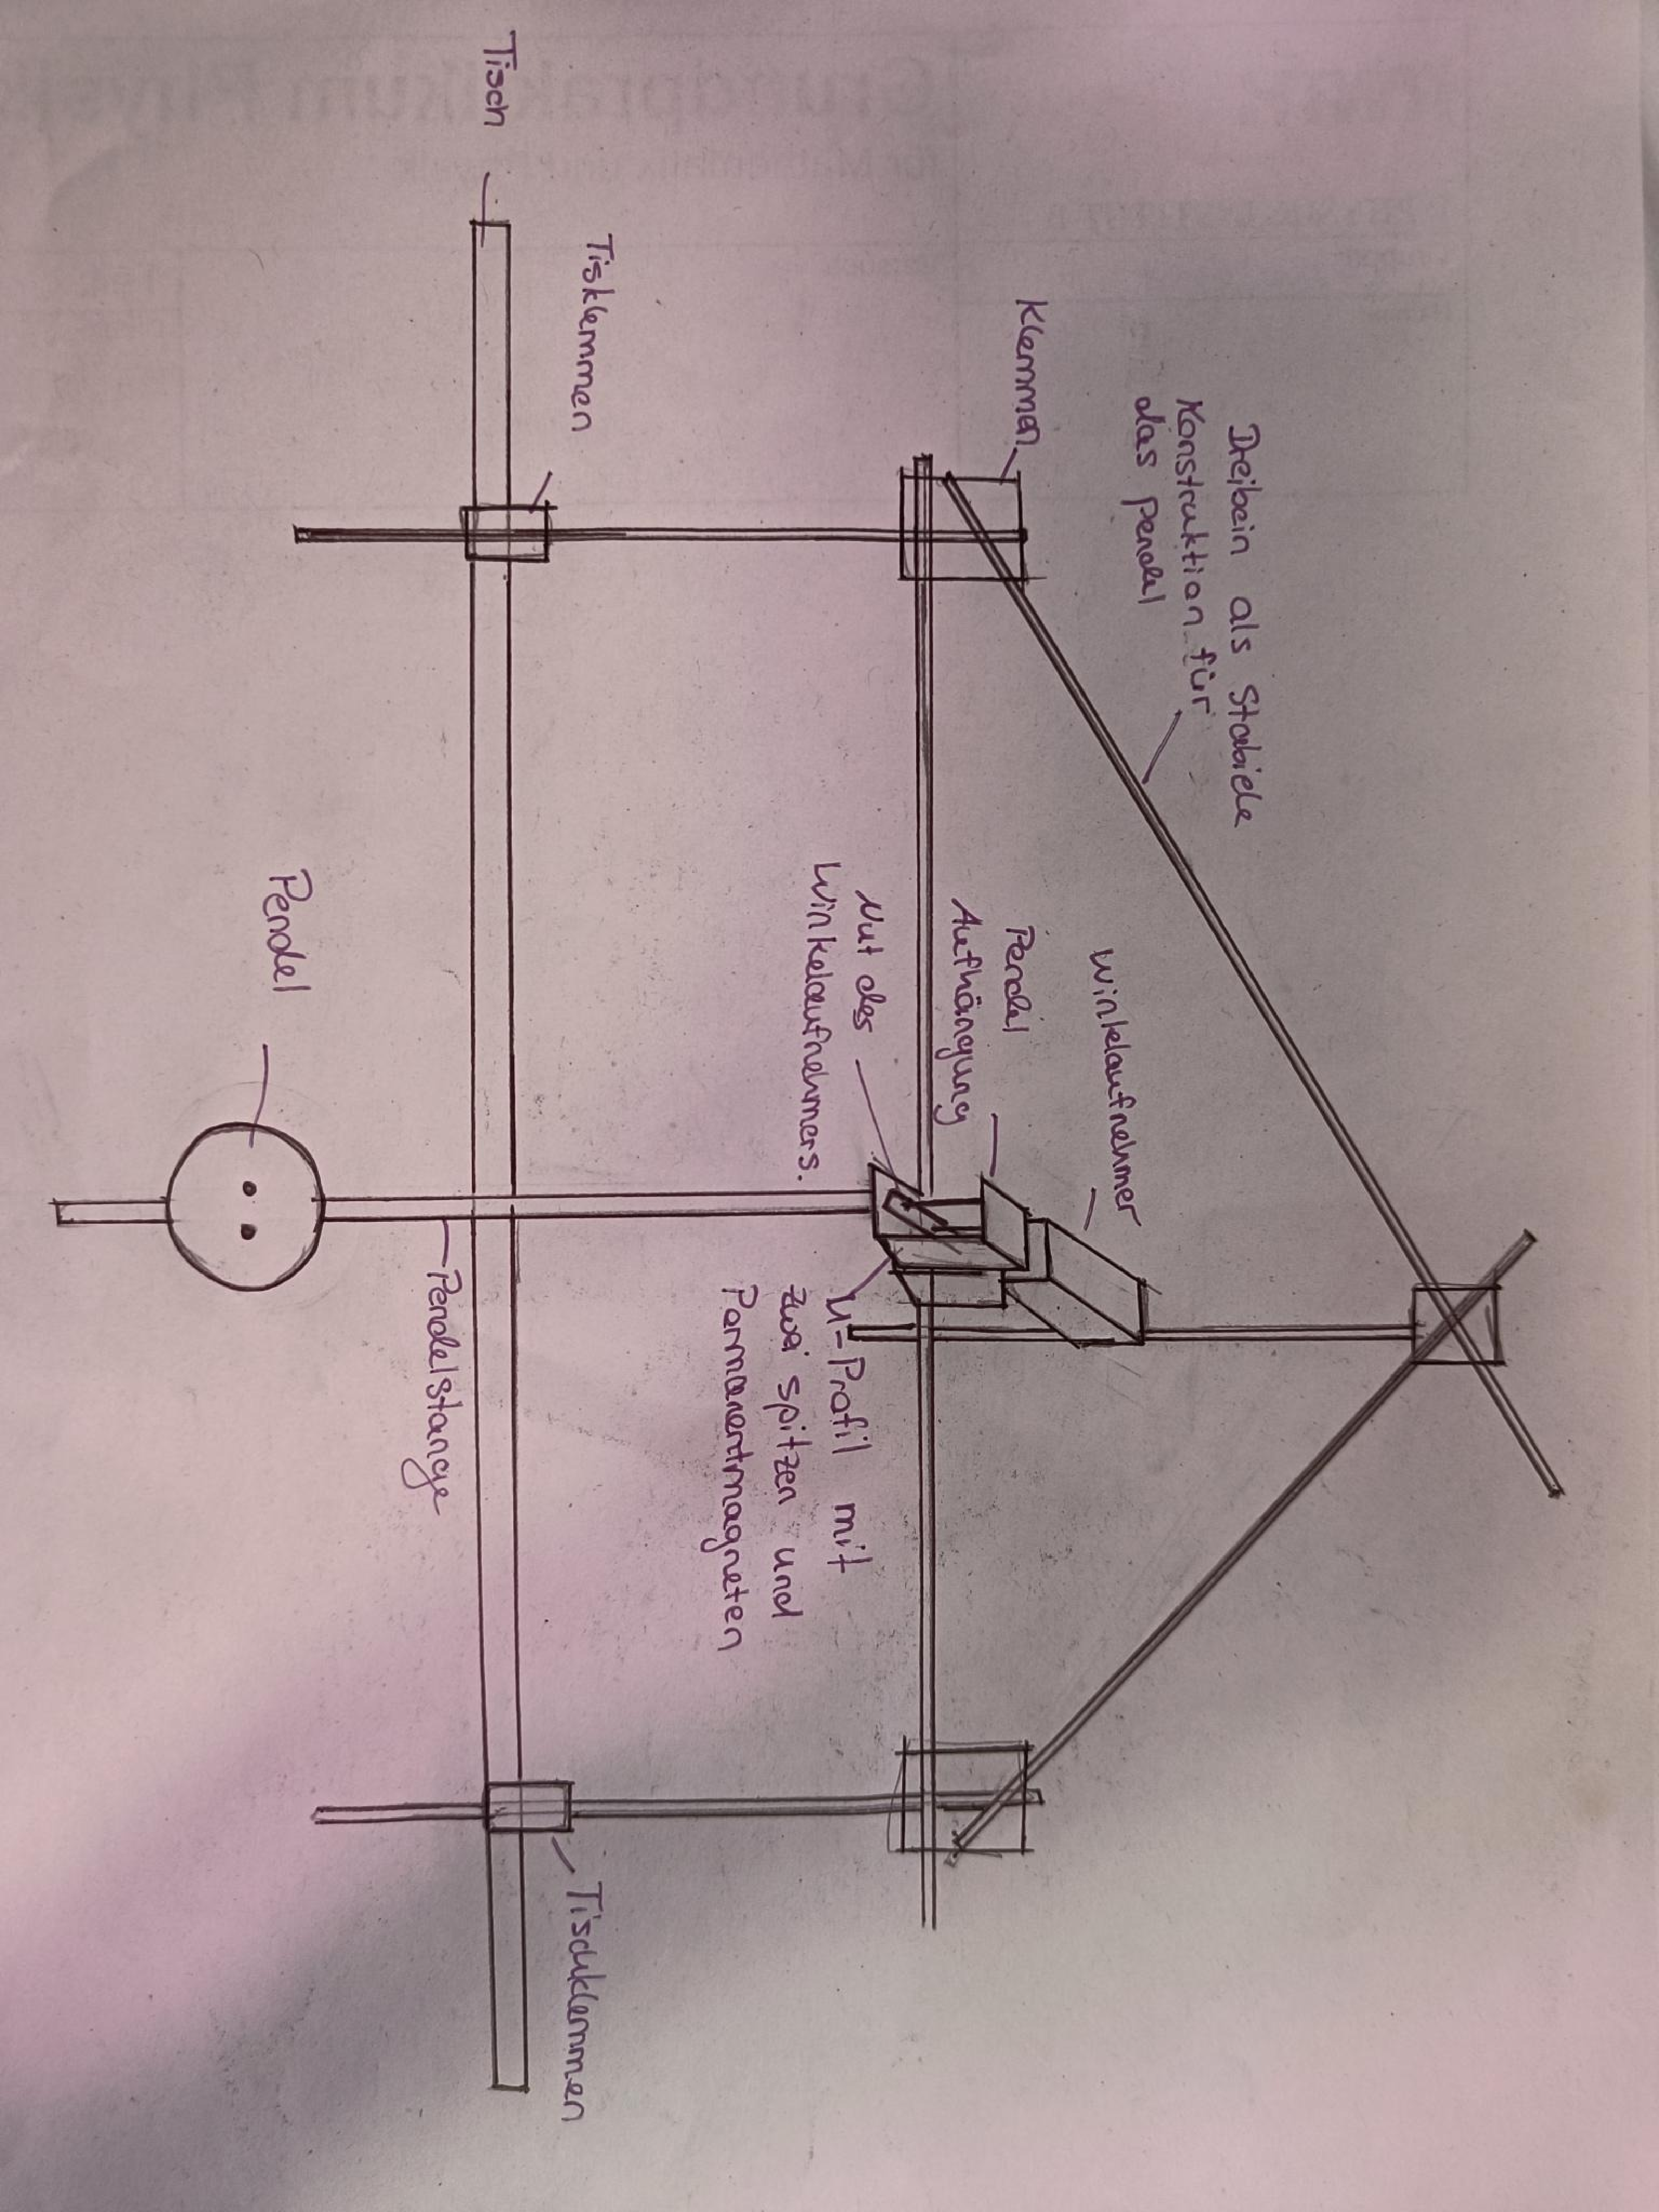
\includegraphics[width=0.7\textwidth]{Bilder/Kompletter-Aufbau.pdf}
    \caption{Nahaufnahme von der Nut mit Nadel}
\end{figure}

Der Oberen Skizze kann der Gesamtaufbau entnommen werden. 
Zunächst werden zwei Tischklemmen mit je einer Stativ Stange am vorne Tisch befestigt.
Die dritte Stativ Stange wird auf der anderen Seite des Tisches in der bereits angebrachten Halterung befestigt. 
Mit Kreuzmuffen (in Skizze mit Klemme beschriftet) werden nun die langen Metallstangen verwendet um diese 3 Stativ Stangen zu verbinden, und so ein Dreieck zu bilden.
Es sollte darauf geachtet, werden, das die Stangen gut in den Kreuzmuffen liegen. 
Bei der vorderen Stange an welcher später das Pendel auf gehangen wird, muss darauf geachtet werden, dass diese horizontal ist.
Dies kann mithilfe der Wasserwaage überprüft werden.\\

Wenn diese Konstruktion stabil ist, kann vorne an der Stange der Winkelaufnehmer befestigt werden. 
Dieser besteht aus einer Stange in welcher 2 Nut sind mit eine Hall-Sonde. 
Dies wird an das CASSY angeschlossen.
Wir haben beide Winkelaufnehmer befestigt, um zu überprüfen welchen wir besser Nullen können, und damit wir später ein Pendel mit und eins ohne Pendelkörper bei der Synchronisation vergleichen können.
Bei den Winkelaufnehmern muss darauf geachtet werden, dass diese fest genug befestigt sind, sodass sich diese nicht verdrehen bei dem Pendelvorgang.\\

Die beide Pendelstangen werden an ein U-Profil geschraubt.
Das U-Profil besteht aus zwei Permanentmagneten die ein homogenes Magnetfeld um die Hall-Sonde erzeugen, Zwei Nadeln auf denen das Pendel schwingen wird, und einer Halterung für die Stange. 
Die zwei Nadeln, werden in die Nut an dem Winkelaufnehmer gestellt.
Der Stellpunkt der Nadeln ist die Rotationsachse des der Pendelschwingung. \\

\begin{figure}[H]
    \centering
    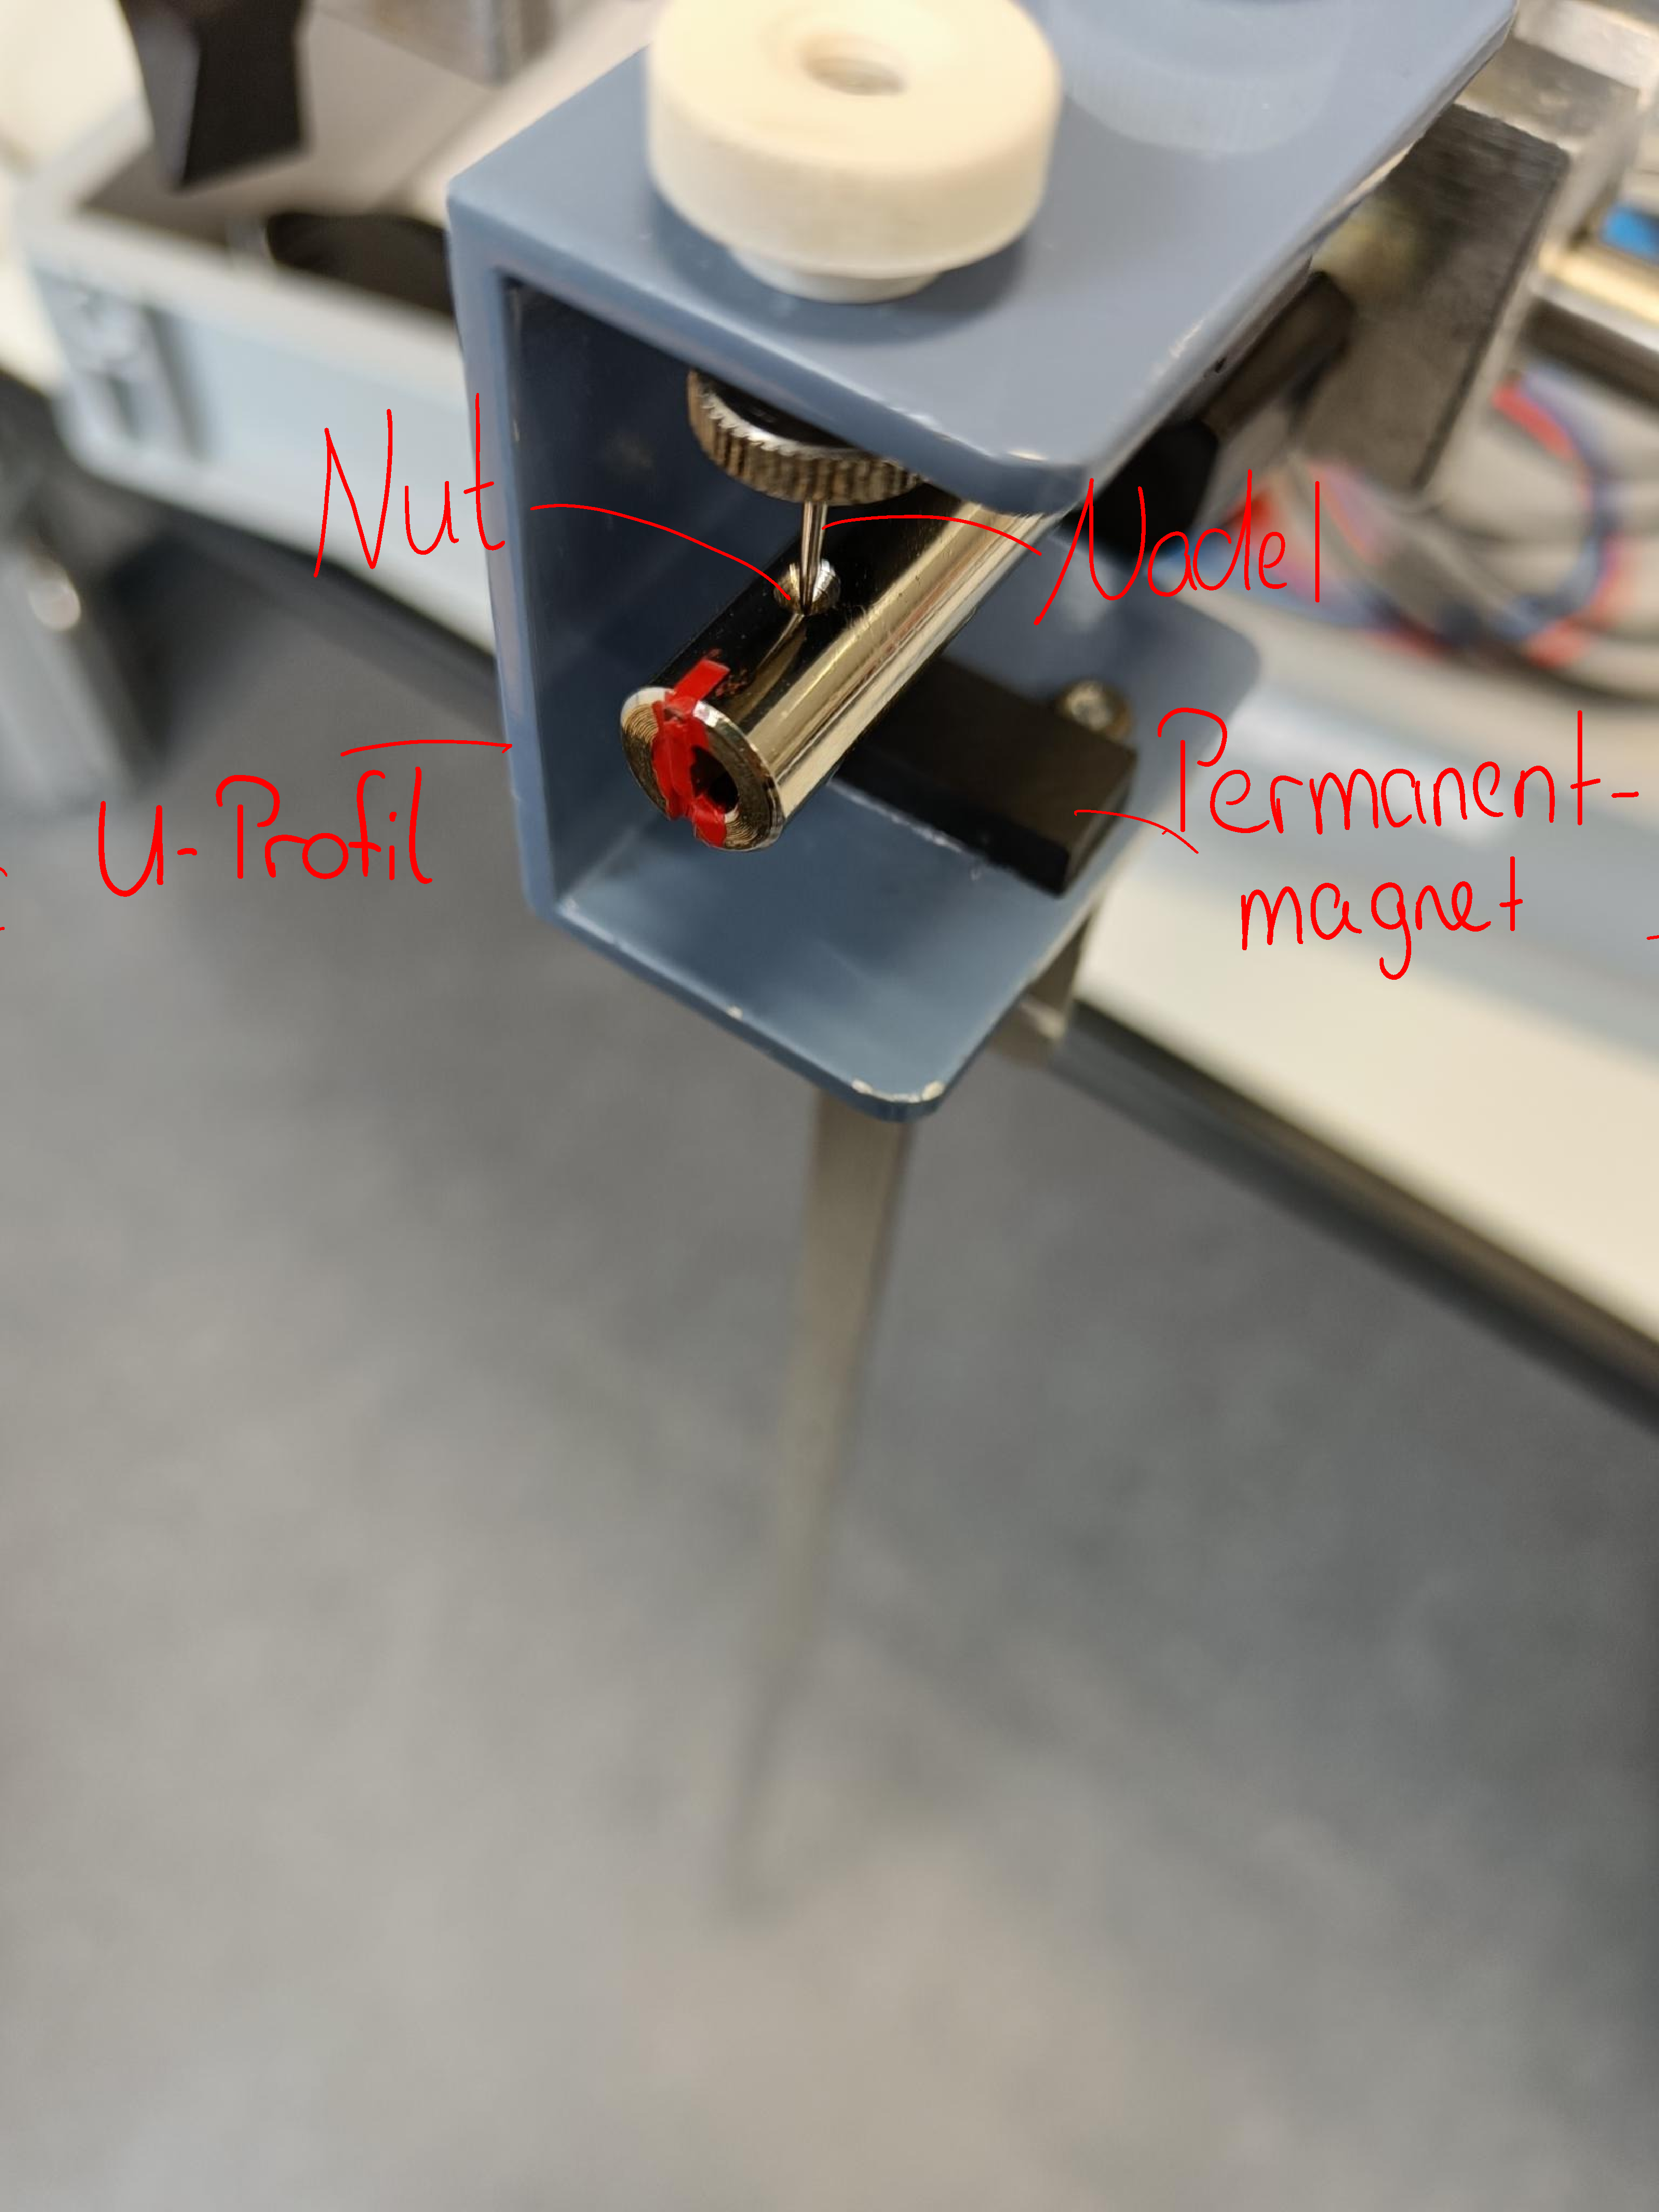
\includegraphics[width=0.7\textwidth]{Bilder/Nahaufnahme-Nut_B.pdf}
    \caption{Nahaufnahme von der Nut mit Nadel}
\end{figure}
In dem Bild oben können sie sehen, wie die Nadel des U-Profils in der Nut des Winkelaufnehmers liegt.

Ein Pendelkörper kann an der Pendelstange befestigt werden, indem man die Stange in diesen schiebt, und mit der Schraube des Pendelkörpers festzieht.\\
\subsection{Durchführung}
Zu beginn des Versuchs haben wir das 3-Bein Stativ aufgebaut wie oben beschrieben. 
Hier sind wir sicher gegangen, dass dieses Fest ist, und haben zur Überprüfung an diesem gewackelt.
Mit der Wasserwaage haben wir überprüft, dass die vordere Stange horizontal ist. 
Dann haben wir beide Winkelaufnehmer mit einer Kreuzmuffe befestigt, Später haben wir diese noch weiter auseinander gerückt, da sich sonst die Pendel in die Quere gekommen wären. 
Mit der Wasserwaage haben wir überprüft, dass der Winkelaufnehmer horizontal ist. 
Diesen haben wir stark befestigt, dass das Gewicht des Pendelkörpers diesen später nicht verdreht.
 
Die Pendelstange haben wir an dem U-Profil mit den davor vorgesehenen Schrauben festgeschraubt, und dieses dann mit den Nadeln in die Nut des Winkelaufnehmers gestellt.\\
Vor beginn der Messung haben wir den Winkelaufnehmer genullt. 
Wir haben beide Winkelaufnehmer an CASSY angeschlossen, um zu überprüfen, welchen wir besser Nullen können.
Hierfür haben wir den Winkelaufnehmer in die Steckdose eingesteckt, und an dem Drehregler des Geräts gedreht, bis bei CASSy ungefähr null Volt angezeigt wurden.
Der auf den Bildern und Skizzen linke Winkelaufnehmer konnten wir besser nullen, weswegen wir diesen für die weiteren Messungen verwendet haben.
Den Winkelaufnehmer haben wir an Input A des CASSY angeschlossen\\
\begin{figure}[H]
    \centering
    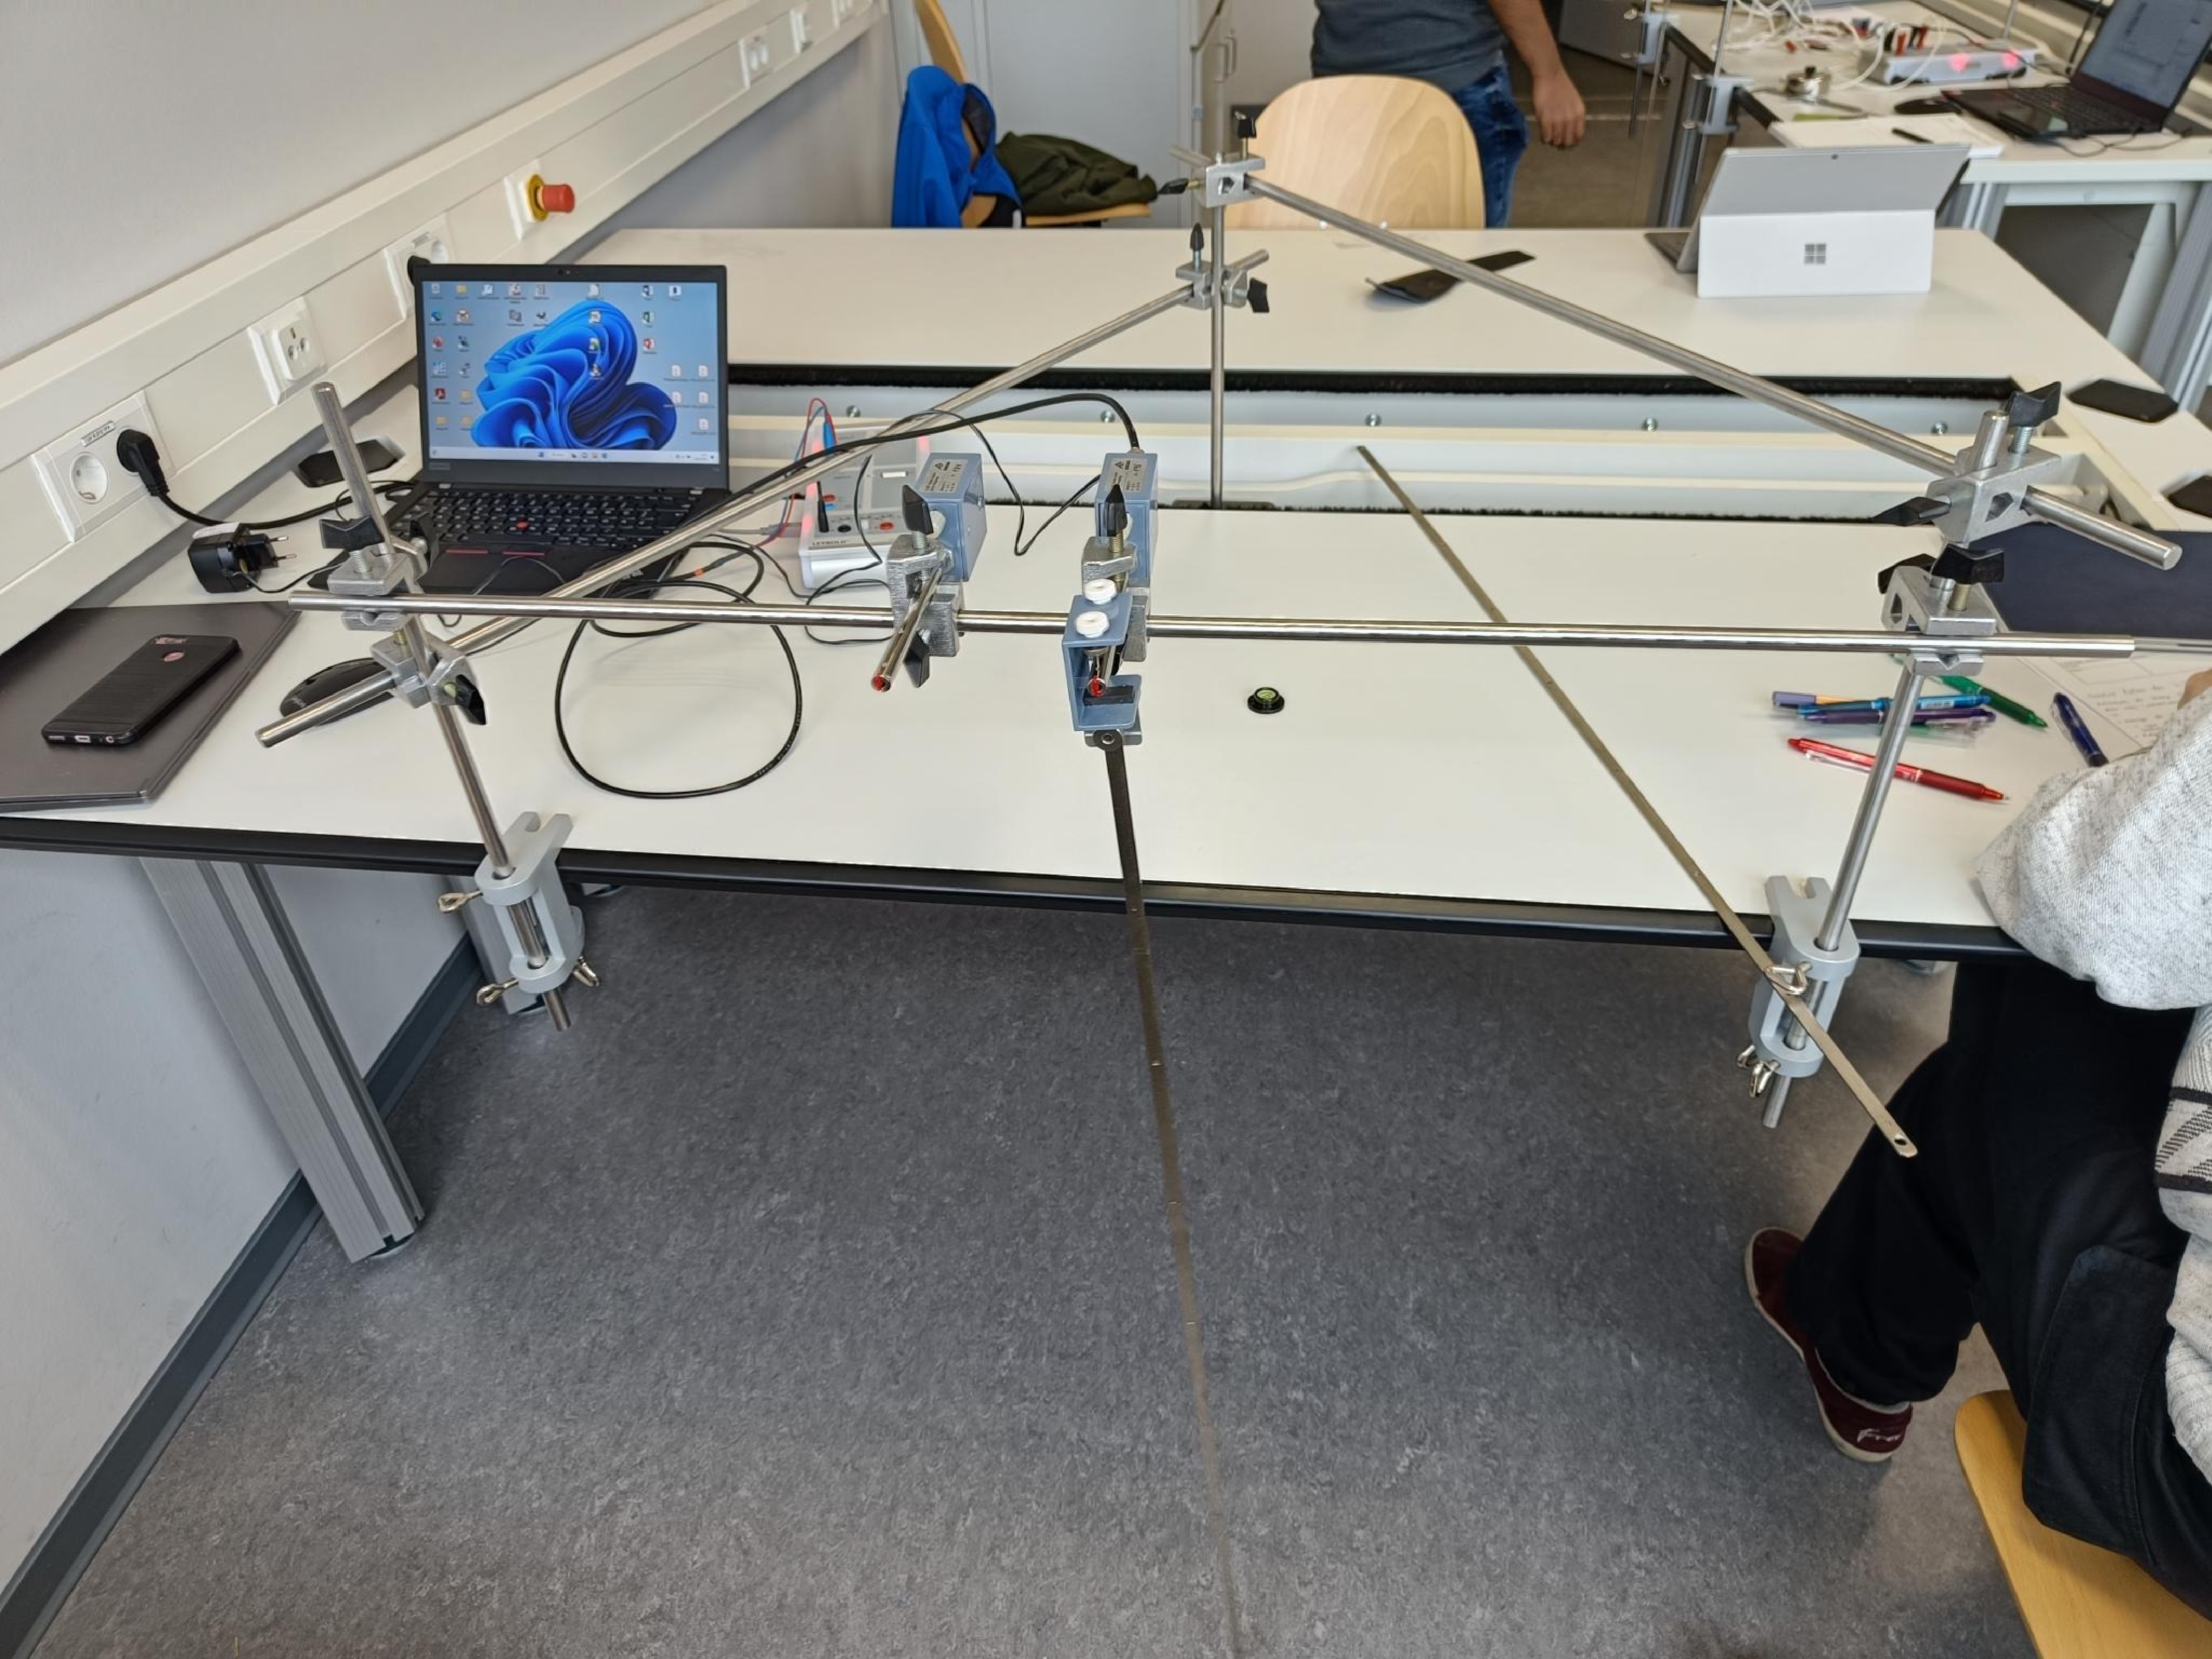
\includegraphics[width=0.7\textwidth]{Bilder/gesamtaufbau.pdf}
    \caption{Bild des Gesamtaufbaus}
    \end{figure}
Hier ein Bild des Gesamtaufbaus. Zu sehen ist das 3-Bein Stativ und das Daran befestigte Pendel.
In diesem betrachten wir das Pendelverhalten der weiten Stange welche wir nicht gewählt haben.\\

Da unsere Kleinwinkelnäherung bis Maximal 5° geht, haben wir ausgerechnet, um welche Strecke am Boden das Pendel ausgelenkt werden darf sodass wir unter 5° bleiben. 
Diese Auslenkung haben wir mit einem Geodreieck auf dem Boden gemessen. 
Die Maximale Auslenkung war 9cm weswegen wir unser Pendel 7cm Ausgelenkt haben.
Bei einer Auslenkung von 7cm hatten wir eine Spannung zwischen -0.4V und 0.4V weswegen wir den Messbereich auf -1V bis 1V gestellt haben.\\

Zur Bestimmung der Messwerterfassungseinstellungen haben wir erst eine Testmessung über wenige Schwingungsperioden durchgeführt, um zu überprüfen wie gut ablesbar die Maxima sind.
Unser erstes Messintervall war 20ms, Mit diesem Konnten wir die Maxima schon gut ablesen, bei einem Messintervall von 10ms war dies jedoch besser.\\
Wir haben ebenfalls die zweite Pendelstange auf gehangen und überprüft wie gut ablesbar bei dieser die Maxima sind.
 Diese waren unsauberer, was daran liegen könnte, dass die Stange gebogen war, und die Schwingung dadurch nicht so gleichförmig abgelaufen ist.
 Diese Vergleichsmessung haben wir unter Test-Vergleich-01 abgespeichert. \\

 Als nächstes haben wir das Pendel in drei Abschnitte eingeteilt in welche wir die Länge des Pendels messen. 
 Die genaue Aufteilung mit Skizze wird in de Rohdaten noch genauer beschrieben. Kurz zusammengefasst messen wir den Abstand zwischen den Nadeln und U-Profil Boden ($l_1$).
Vom U-Profil Boden bis zur ersten Einkerbung der Pendelstangen Halterung ($l_2$) und von dort bis zum Mittelpunkt des Pendelkörpers ($l_3$).
$l_1$ und $l_2$ sind Strecken die gut mit dem Messschieber gemessen werden können, da man diese gut ansetzen kann. 
Von der ersten Einkerbung konnte man das Maßband gut hängen lassen.
Für $l_1$ und $l_2$ haben wir die Messungen vor dem Pendeln durchgeführt. 
Wir haben jede Strecke 3 mal gemessen. Den Abstand zwischen Nadel und U-Profil Boden haben wir pro Nadel 3 mal gemessen.\\

Dann haben wir die erste Messung gestartet. 
Die Messung haben wir Manuell gestartet, also ohne Trigger, sodass wir anfängliche Störungen vom Auslenken des Pendels nicht aufzeichnen. 
Wir haben jede Messung von Hand abgebrochen nach ca. 185 Sekunden. 

\begin{table}[H]
        \centering
        \begin{tabularx}{1.0\textwidth}{X X X X} % adjust width as needed
            \toprule
            \textbf{Intervall} & \textbf{Messzeit} & \textbf{Trigger} & \textbf{Bereich} \\
            \midrule
            1ms & 185s & kein Trigger & -1V bis 1V \\
            \bottomrule
        \end{tabularx}
        \caption{Messwerterfassungseinstellungen}
        \label{tab:mytable}
    \end{table}

Hier eine Übersicht unserer Messwerterfassungseinstellungen.\\
Das Penel haben wir mit der Hand ca. 7cm ausgelenkt, dies haben wir mit dem Geodreieck gemessen (Auf Bild unten zu sehen). 
Bei jeder Messung haben wir versucht in etwa die gleiche Auslenkung zu haben. 
Das pendel sollte möglichst störungsarm losgelassen werden, um mögliche Effekte des Starten zu minimieren. 
Falls das Pendel zu sehr hin und her gewackelt hat, haben wir die Messung abgebrochen und neu gestartet.\\
\begin{figure}[H]
    \centering
    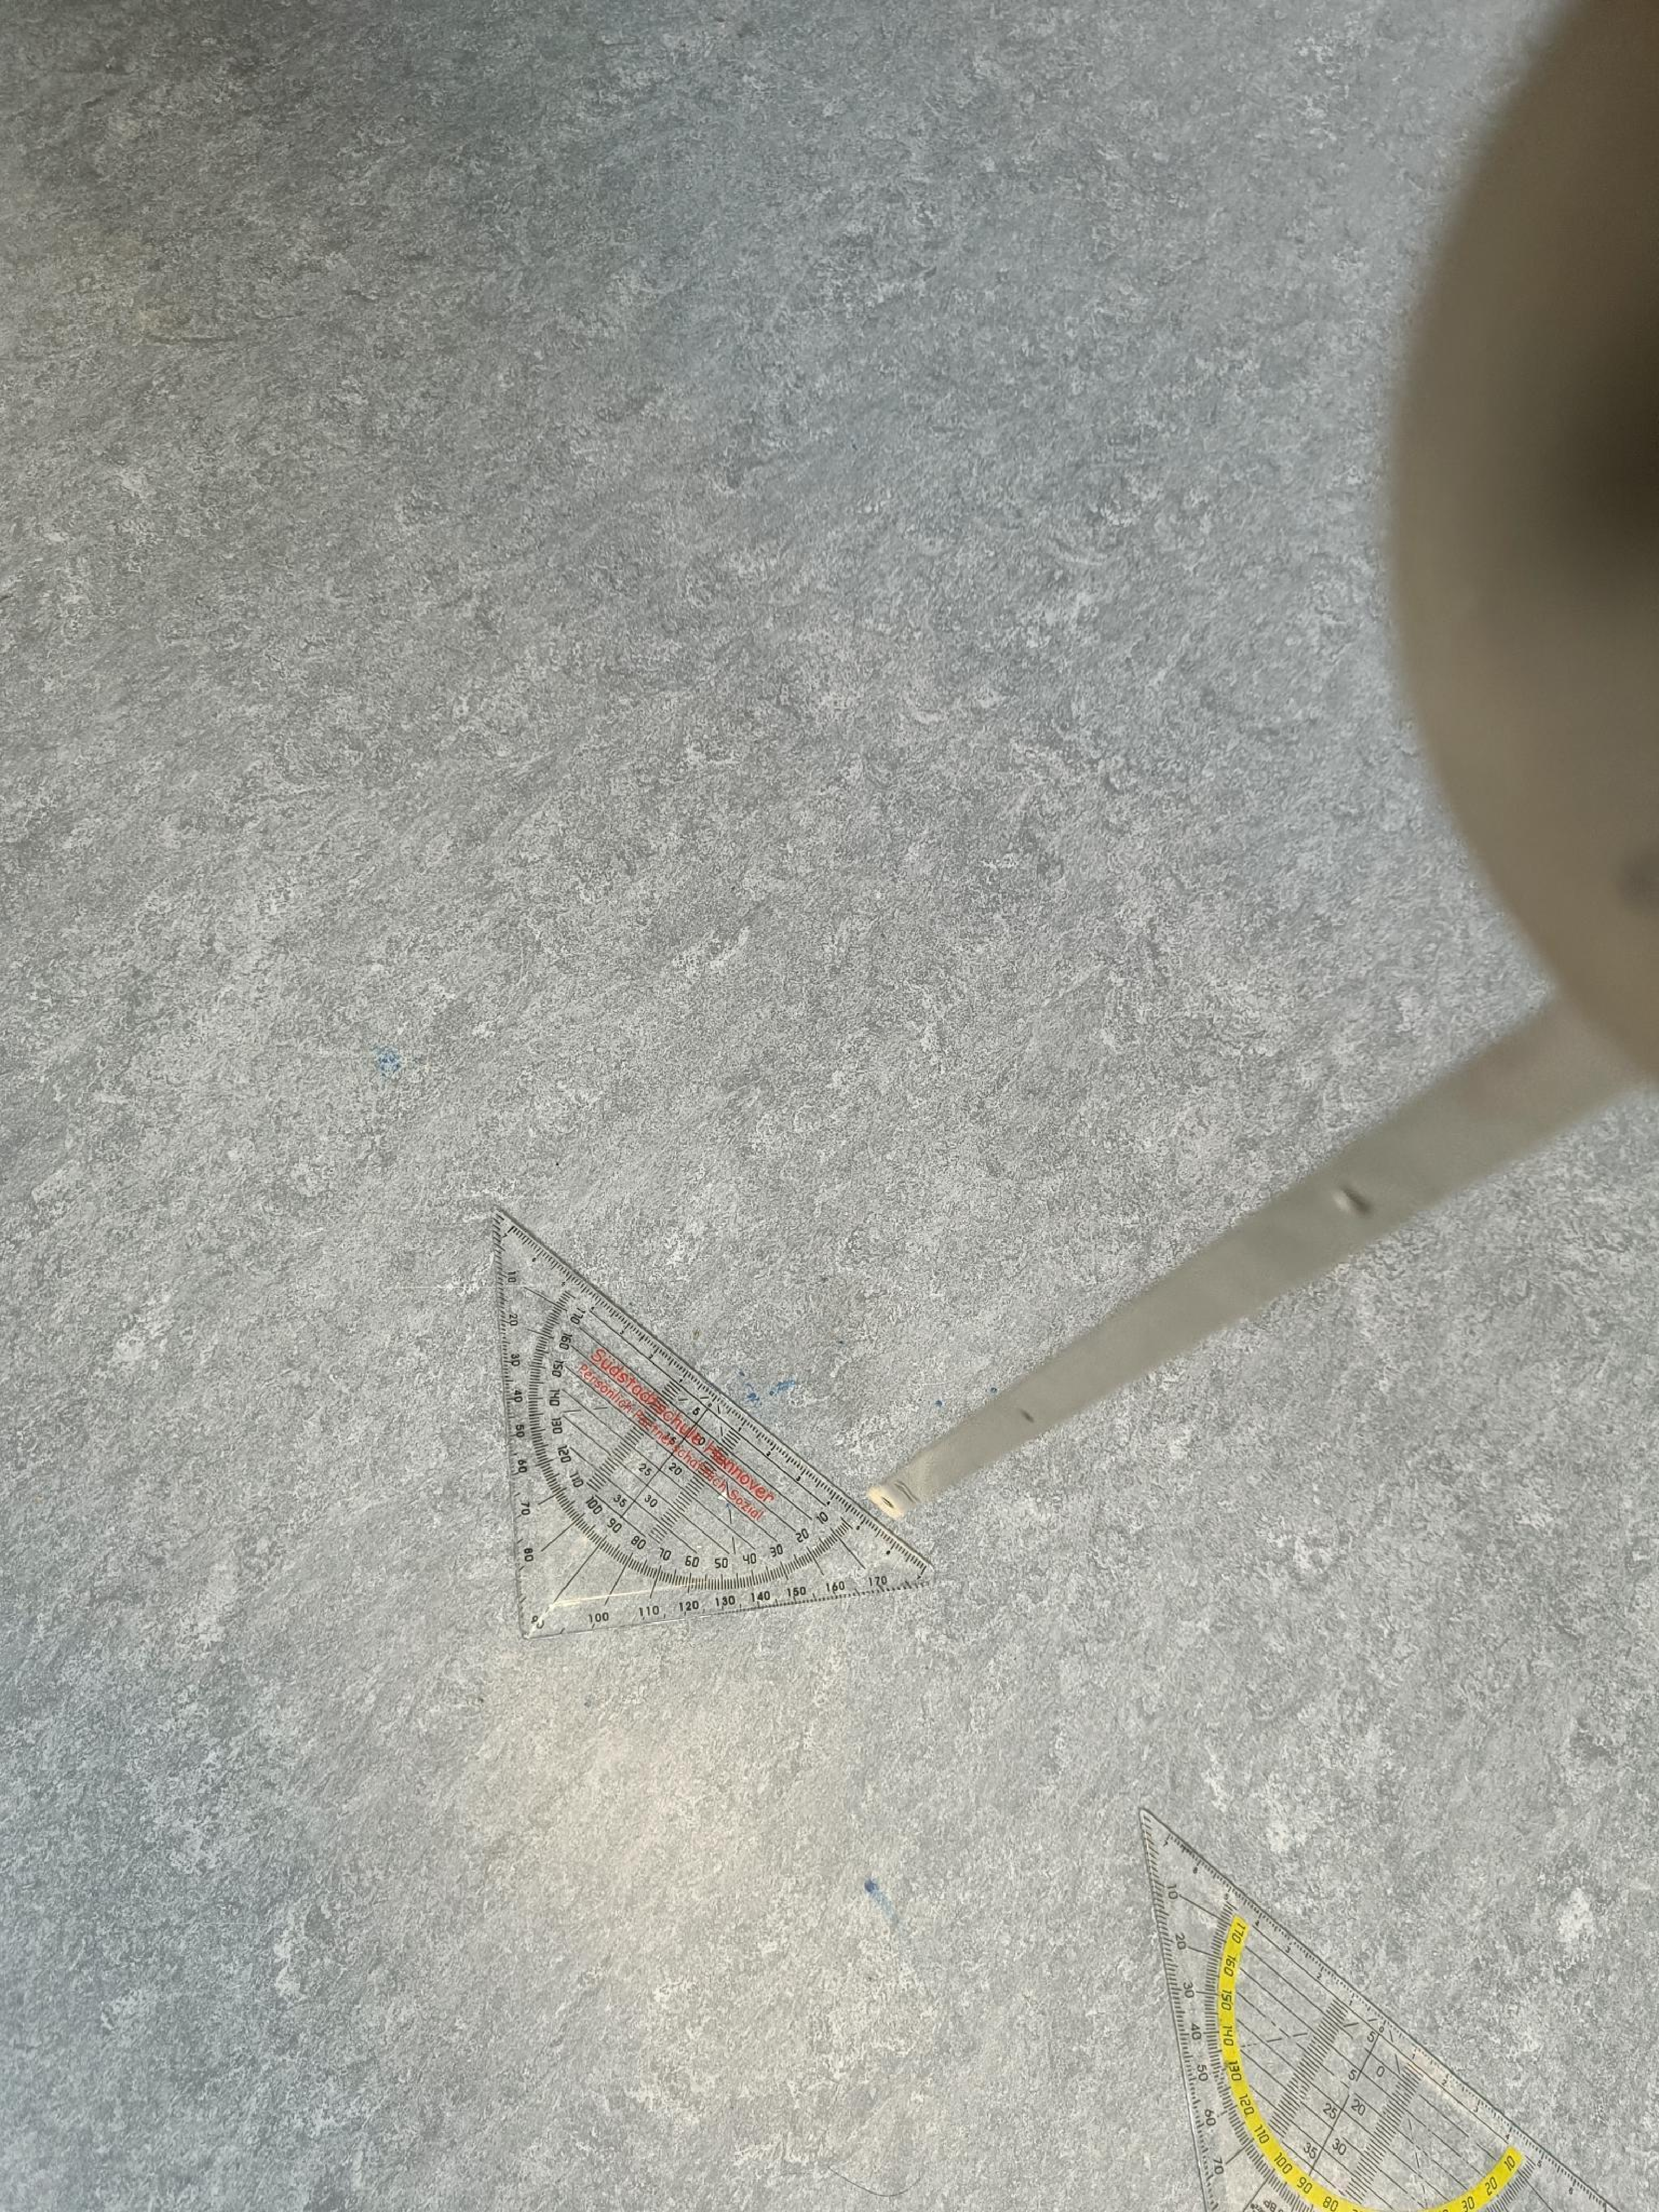
\includegraphics[width=0.7\textwidth]{Bilder/geodreieck.pdf}
    \caption{Bestimmung der Auslenkung mit Geodreieck}
    \end{figure}
Die Messung nur mit der Pendel Stange haben wir insgesamt drei mal durchgeführt. 
Für jede dieser Messungen haben wir die Periodendauer überschlagen.
Wir haben den Zeitpunkt des ersten Maximums mit dem Peakschwerpunkt bestimmt. Das selbe haben wir mit dem zwanzigsten Maximum getan. 
Die Periodendauer haben wir dann mit der folgenden Formel bestimmt.
\begin{equation}
T = \frac{t_{20} - t_{1}}{19}
\end{equation}
Bei der Rechnung nach nach der Messung haben wir durch die falsche Periodenzahl (20) geteilt. 
Dies ist uns aufgefallen, als wir g bestimmt haben, weshalb wir unsere Rechnungen für die Periodendauer wiederholt haben.\\

Nachdem wir diese durchgeführt haben, haben wir den Pendelkörper an der Pendelstange befestigt. 
Und das Pendel erneut auf gehangen. 
Diesmal waren wir beim aufhängen besonders vorsichtig, das die Masse des Pendels nun um einiges größer war, und somit den Winkelaufnehmer verdrehen könnte
An den anderen Winkelaufnehmer haben wir die andere Pendelstange gehangen, und beide Pendel ausgelenkt.
Nach Augenmaß haben wir überprüft, ob diese ungefähr die gleiche Frequenz haben. Und haben gegebenenfalls Die Position des Pendelkörpers angepasst.
Wenn dass Pendel mit Pendelkörper eine kleinerer Periodendauer hat, muss der Pendelkörper nach unten bewegt werden, wenn es eine größere Periodendauer hat nach oben.
Diese Justierungen haben wir durchgeführt, bis die Frequenz augenscheinlich übereingestimmt hat. \\

Danach haben wir mit CASSY einige Schwingungsperioden (zwischen 10 und 50) aufgenommen um zu überprüfen, ob die Frequenzen der beiden übereinstimmen. 
Hierfür haben wir die Lage der Maxima der beiden Schwingungen (Schwingung mit Pendelkörper und ohne) verglichen.
Ob deren relative position zueinander im Verlauf der Messung gleich geblieben ist.
Hier haben wir den Pendelkörper ebenfalls einige male neu justiert und den Vergleich erneut durchgeführt bis die relative Position der Maxima gleich geblieben sind.\\

Mit dieser Pendelkörperposition haben wir dann eine gesamte Messung durchgeführt.
Dies haben wir gleich wie bei dem Pendel ohne Pendelkörper gemacht. Wir haben wieder 185 Sekunden aufgezeichnet. 
Daraus haben wir ebenfalls die Periodendauer überschlagen. 
Dies haben wir auf die gleiche weise getan wie ohne Pendelkörper. Wobei wir wieder durch 20 geteilt haben.
Da die Periodendauern übereingestimmt haben, haben wir mit dieser Position zwei weitere Messungen durchgeführt.
Für diese haben wir jedes mal die Periodendauer überschlagen.\\

Zur Messung des Durchmessers, haben wir das Pendel vom Winkelaufnehmer genommen und mit dem Messschieber den Durchmesser gemessen.
Wir haben darauf geachtet, dass sie möglichst mittig positioniert war, und wir in drei verschiedenen Positionen gemessen haben. \\

Den Abstand vom Pendelkörpermittelpunkt bis zu der ersten Einkerbung der Pendelaufhängung haben wir in hängendem Zustand mit dem Maßband gemessen ($l_3$).
Wir haben das Maßband gerade runter hängen lassen sodass es nicht gebogen ist. 
Durch die Messung mit dem Messschieber wussten wir, dass der Mittelpunkt 4.040cm unter der oberen Kante war.
Wir haben die Position das Maßband sowohl nach Augenmaß mit dem Mittelpunkt verglichen, als auch geschaut, 
dass der Punkt an welchem wir ablesen 4.040cm unterhalb dem oberen Pendelkörper Rands ist.

Auch diese Messung haben wir drei mal durchgeführt.\\
Im Nachhinein ist uns aufgefallen, dass dies keine sehr geschickte Wahl war, da wir eh den Radius des Pendelkörpers mit der Messschieber bestimmt haben.
Eine höhere Genauigkeit hätten wir erzielen können, wenn wir nur bis zu der Oberseite des Pendels gemessen hätten. 

Zuletzt haben wir dann eine Überschlagsrechnung für g gemacht. Dies haben wir mit Formel \ref{eq:formel} gemacht.
Da wir kein sinnvolles Ergebnis erhalten haben, ist uns aufgefallen, dass in der Vorherigen Berechnung von T einen Fehler gemacht haben. 
So konnten wir unsere Rechnung für T korrigieren und g erneut bestimmen. Da dieses Ergebnis mit unseren Erwartungen (von ca. 9.81$m/s^2$) übereinstimmt haben wir den Versuch beendet.

\begin{aufgabe}{Rohdaten}
  Stellen Sie Ihre Rohdaten dar, tabellarisch für $l_p$ und $r_p$,
  grafisch für den Verlauf der Schwingung der Stange ohne Pendelkörper
  sowie der Pendelschwingung (für mindestens drei Messreihen).
\end{aufgabe}

\section{Rohdaten}
Zur Bestimmung der Pendellänge haben wir das Pendel in verschiedene Teilstücke unterteilt, damit wir diese Möglichst genau messen können. 
Dies Abschnitte haben wir so gewählt, dass wir diese mit dem jeweiligen Messinstrument möglichst exakt bestimmen können. 

\begin{figure}[H]
    \centering
    \subfloat[Skizze U-Profil mit Längenabschnitten]{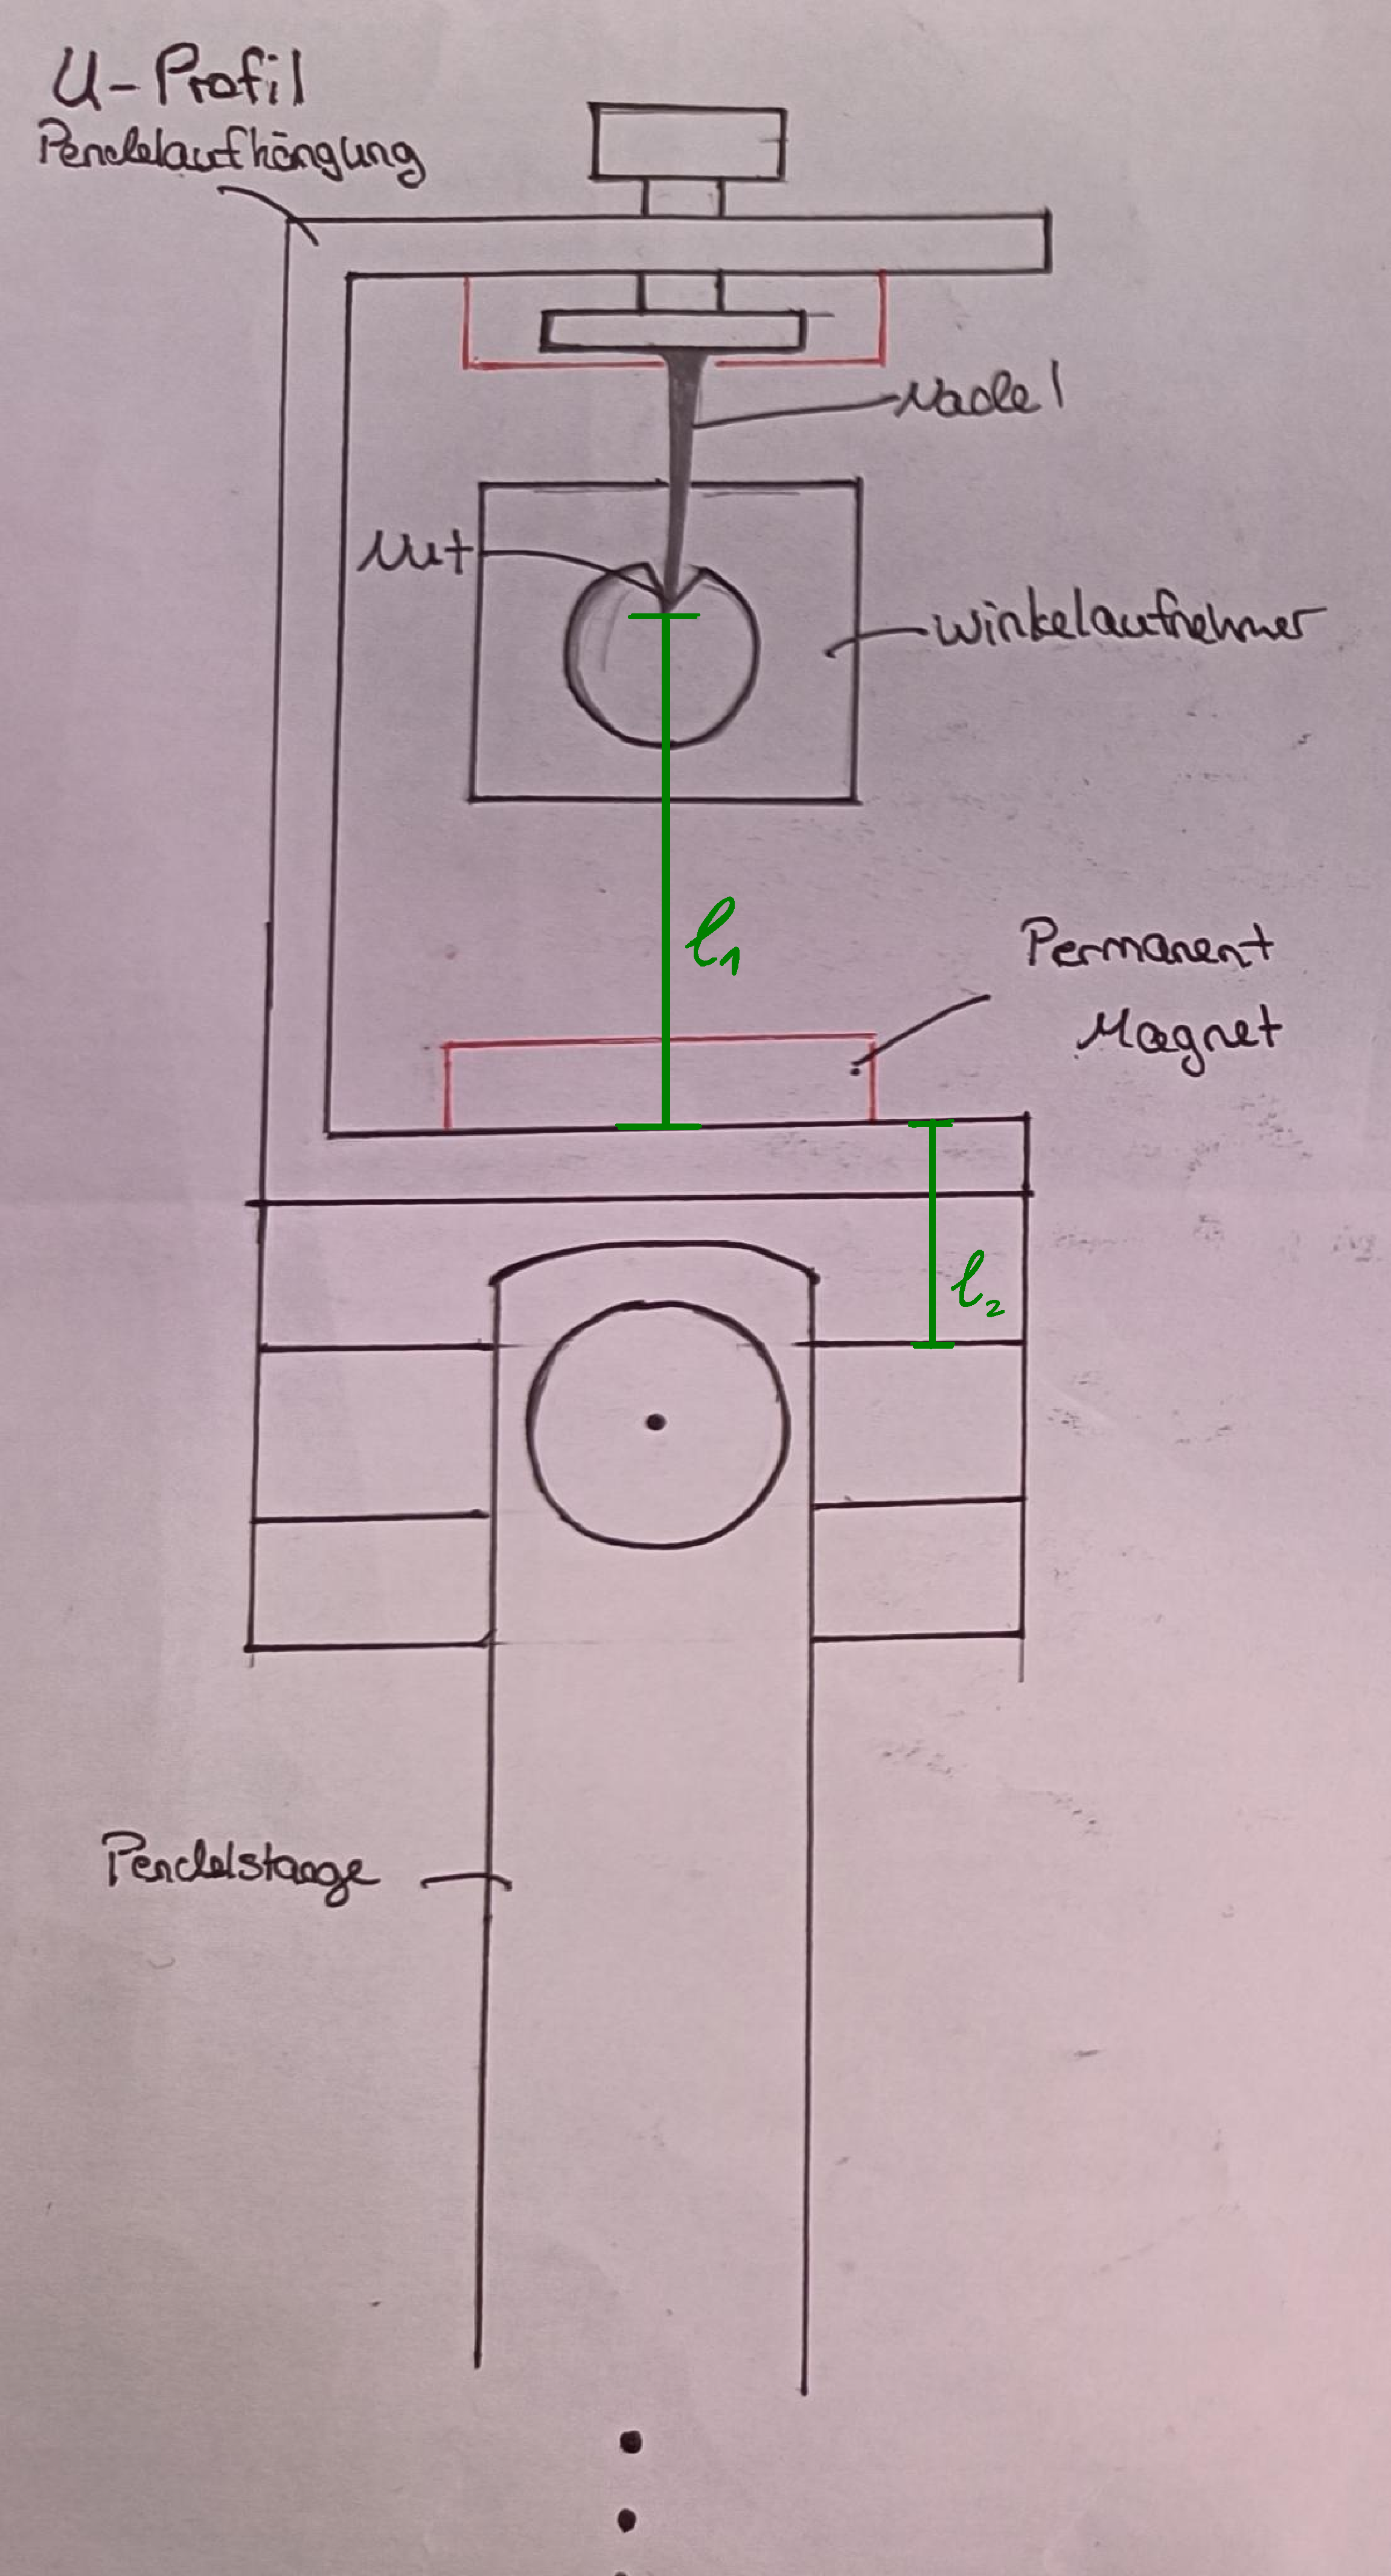
\includegraphics[width=0.45\textwidth]{Bilder/u-profiel-L.pdf}}
    \hfill 
    \subfloat[Skizze des Gesamten Pendel mit Längenabschnitten]{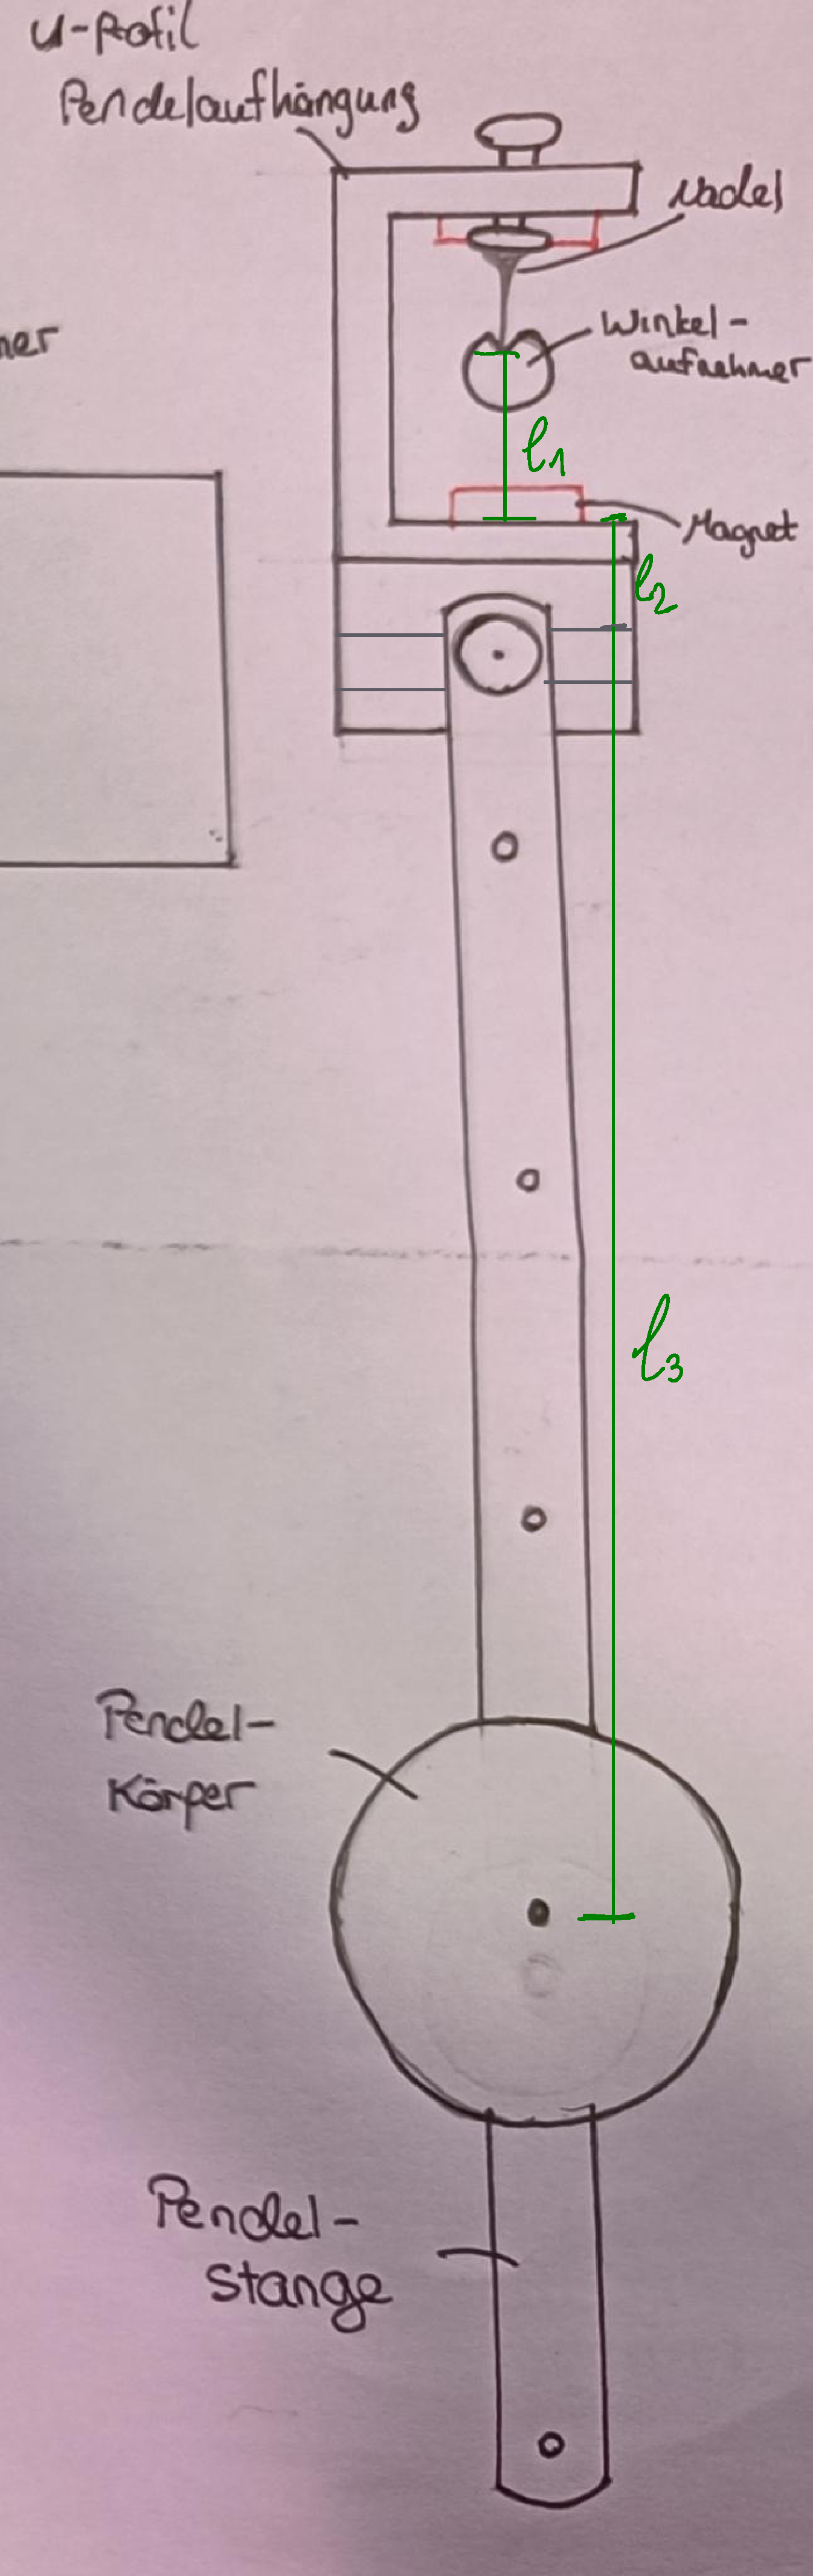
\includegraphics[width=0.3\textwidth]{Bilder/pendel-gesamt-L.pdf}}
\end{figure}
In den Beiden Skizzen ist zu sehen wie wir die Längenabschnitte gewählt haben. 
Hier ist zu beachten, dass die Zeichnung nicht Maßstabsgetreu ist.
$l_1$ ist der Abstand zwischen Nadelspitze und dem Boden des U-Profils. 
Dies haben wir mit der Schieblehre gemessen, wären die Pendelstange noch nicht montiert war und das U-Profil nicht auf gehangen.\\

$l_1$ bezeichnet den Abschnitt zwischen dem Boden des U-Profils und der ersten Einkerbug der Pendelaufhängung.
$l_2$ ist der Abstand zwischen der Ersten Einkerbung bis zum Mittelpunkt des Pendelkörpers.\\ 

Da dad U-Profil zwei Nadeln hat, haben wir von jeder jeweils den Abstand zum Boden gemessen. 
Die eine Messung bezeichnen wir als $l_1$ die andere als $l_4$.
\begin{figure}[H]
    \centering
    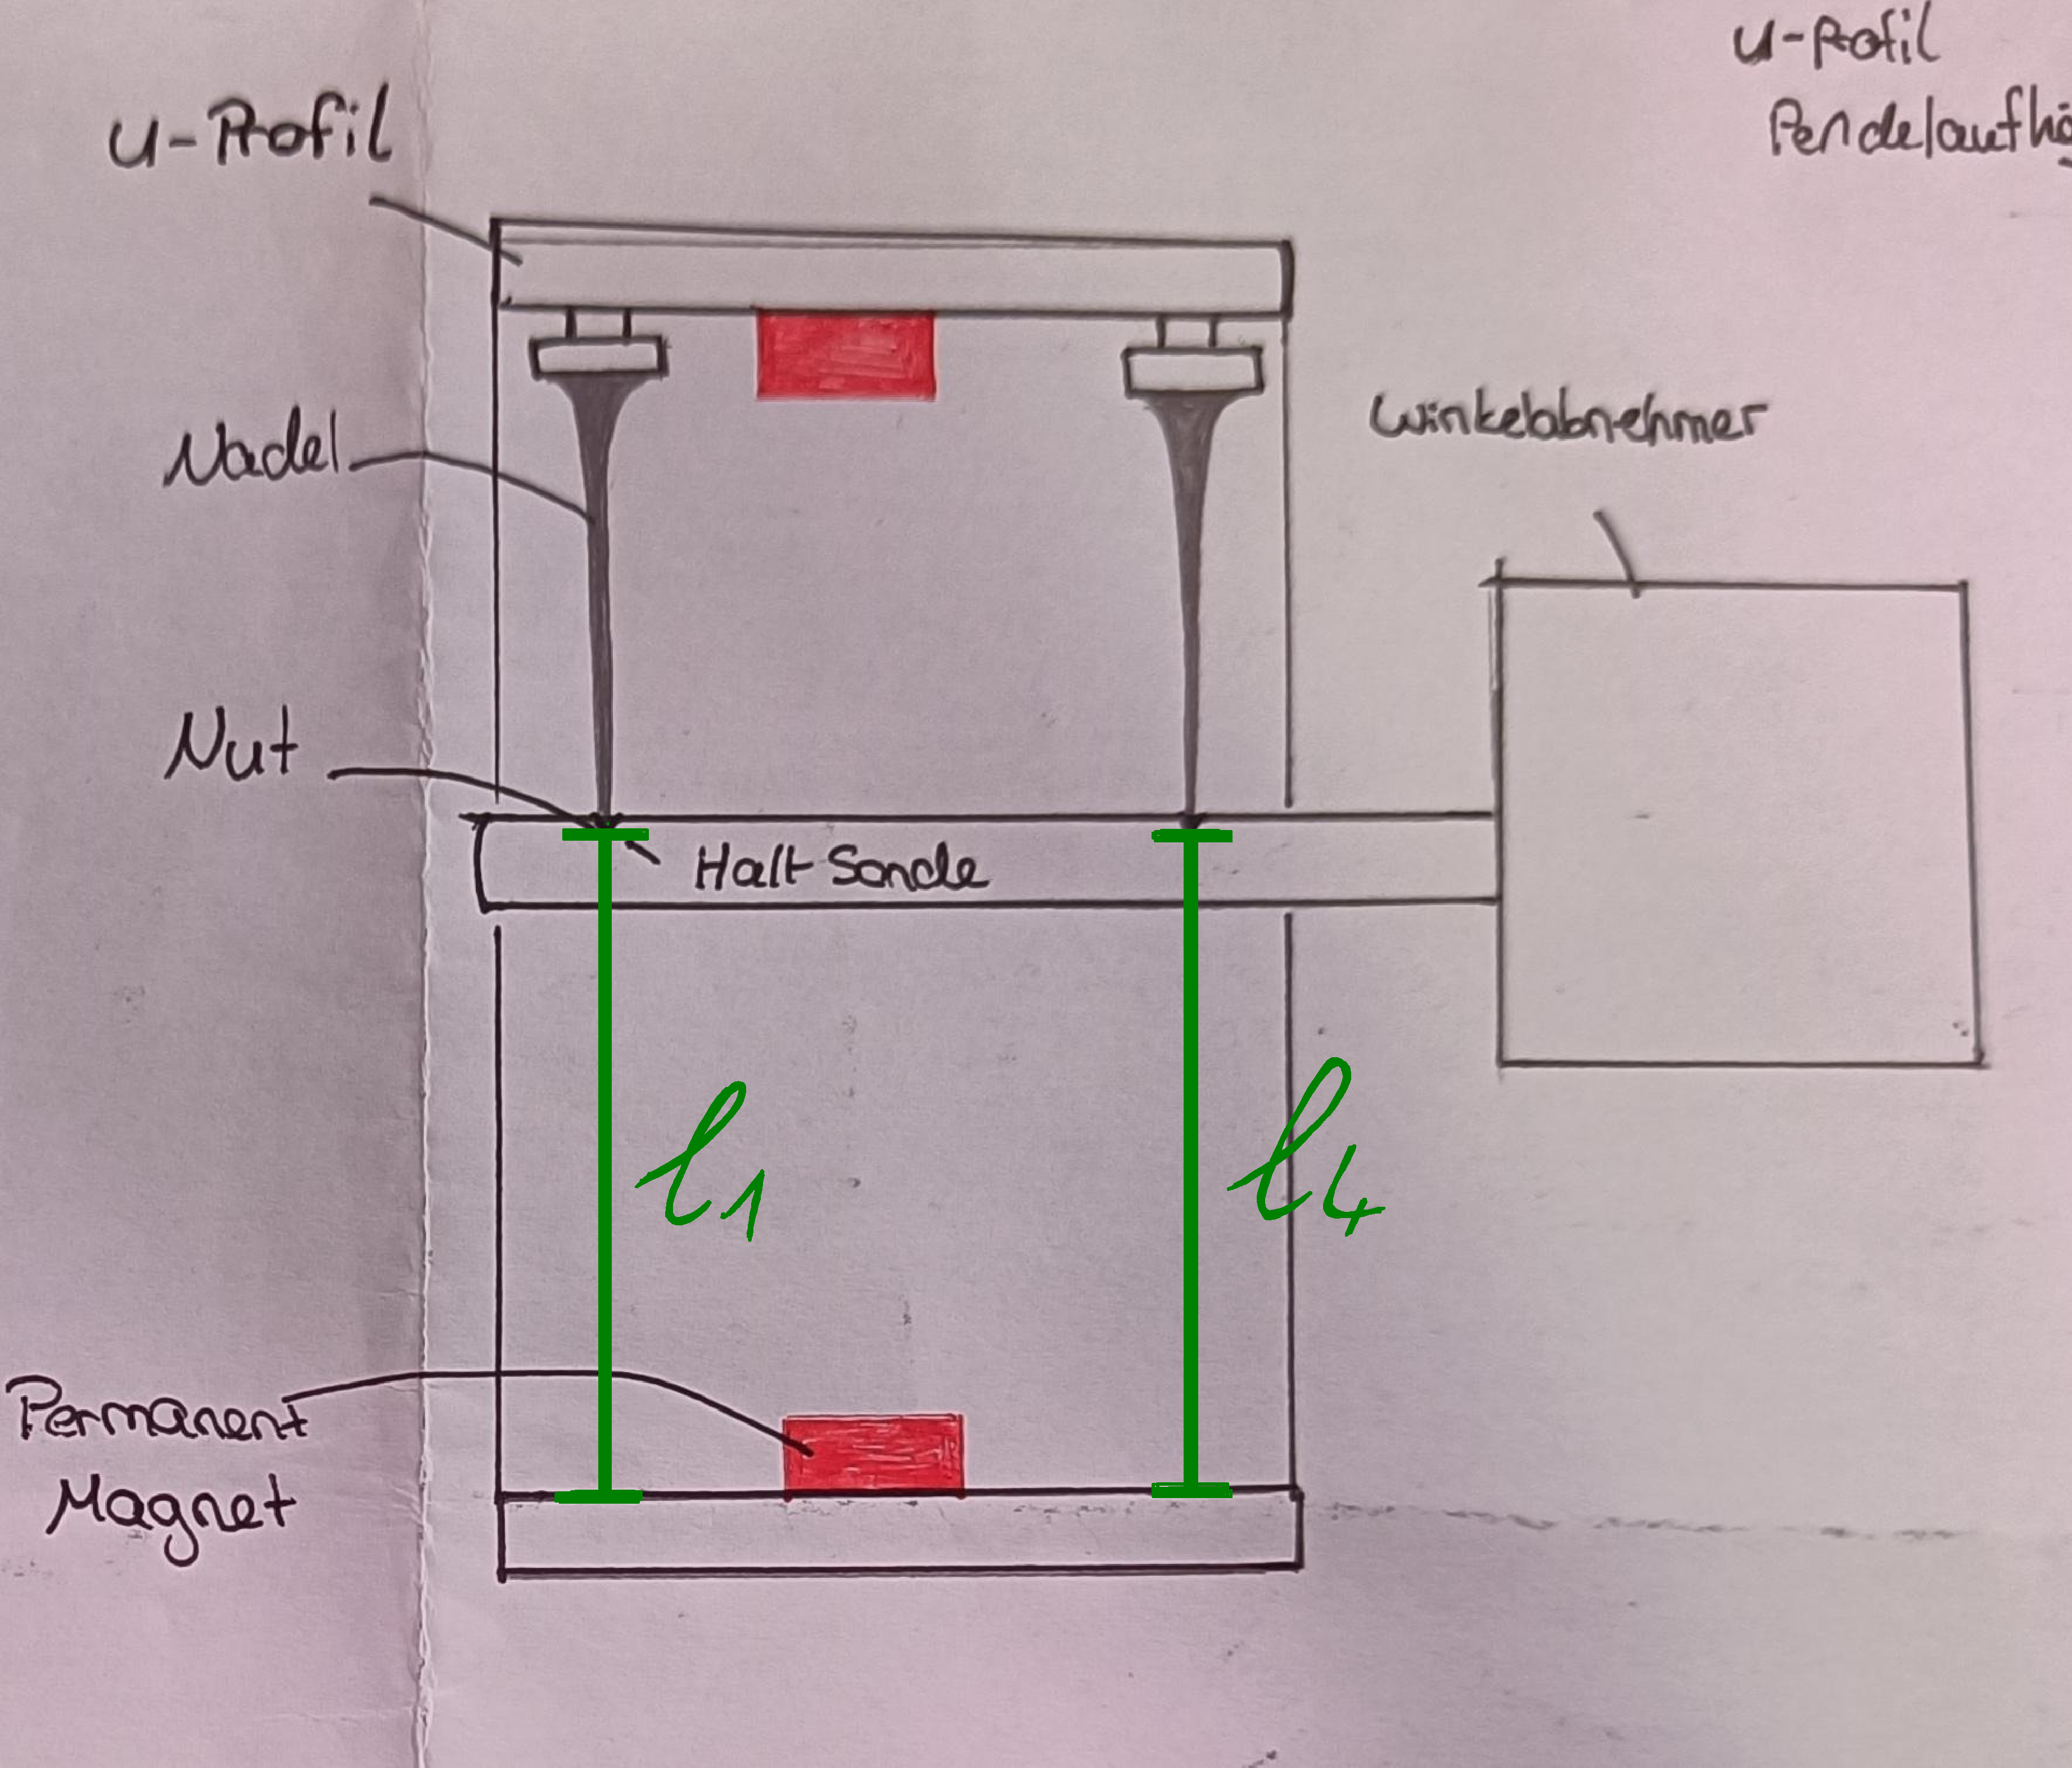
\includegraphics[width=0.45\textwidth]{Bilder/auflage-pende-L.pdf}
    \caption{Skizze des U-Profils mit beiden Nadeln und den Längenabschnitten}
\end{figure}

Für den Radius des Pendelkörpers haben wir den Durchmesser ($d_p$) von diesem bestimmt.
Auf diese Längenmessungen gibt es auch Fehler, hier liegen sowohl systematische Fehler als auch statistische Fehler vor.
Die Systematischen Fehler können den Herstellerangaben entnommen werden für die Messschieber und für das Maßband.
Die statistischen Fehler können aus der Ablesegenauigkeit bestimmt werden. Diese Fehler werden in der Auswertung genauer diskutiert. 


\begin{table}[H]
        \centering
        \begin{tabularx}{1.0\textwidth}{X l X X} % adjust width as needed
            \toprule
            \textbf{Messung} & \textbf{Längenabschnitt} & \textbf{Wert in cm} & \textbf{Messinstrument} \\
            \midrule
            1. & $l_1$ & 2.595 & Messschieber \\
            2. & & 2.590 &\\ 
            3. & & 2.585 &\\
            \midrule
            1. & $l_2$ & 1.110 & Messschieber \\
            2. & & 1.110 &\\
            3. & & 1.110 &\\
            \midrule
            1. & $l_3$ & 64.3 & Maßband \\
            2. & & 64.4 &\\
            3. & & 64.3 &\\
            \midrule
            1. & $l_4$ & 2.600 & Messschieber \\
            2. & & 2.605 &\\
            3. & & 2.605 &\\
            \midrule
            1. & $d_p$ & 8.080 & Messschieber \\
            2. & & 8.080 &\\
            3. & & 8.080 &\\
            \bottomrule
        \end{tabularx}
        \caption{Tabelle der Längenmessungen}
        \label{tab:längen}
    \end{table}
     
Die Messung der Schwingung ohne Pendelkörper, haben wir insgesammt drei mal durchgeführt.
Für jede haben wir die Schwingungsverläufe aufgezeichnet.
\begin{figure}[H]
    \centering
    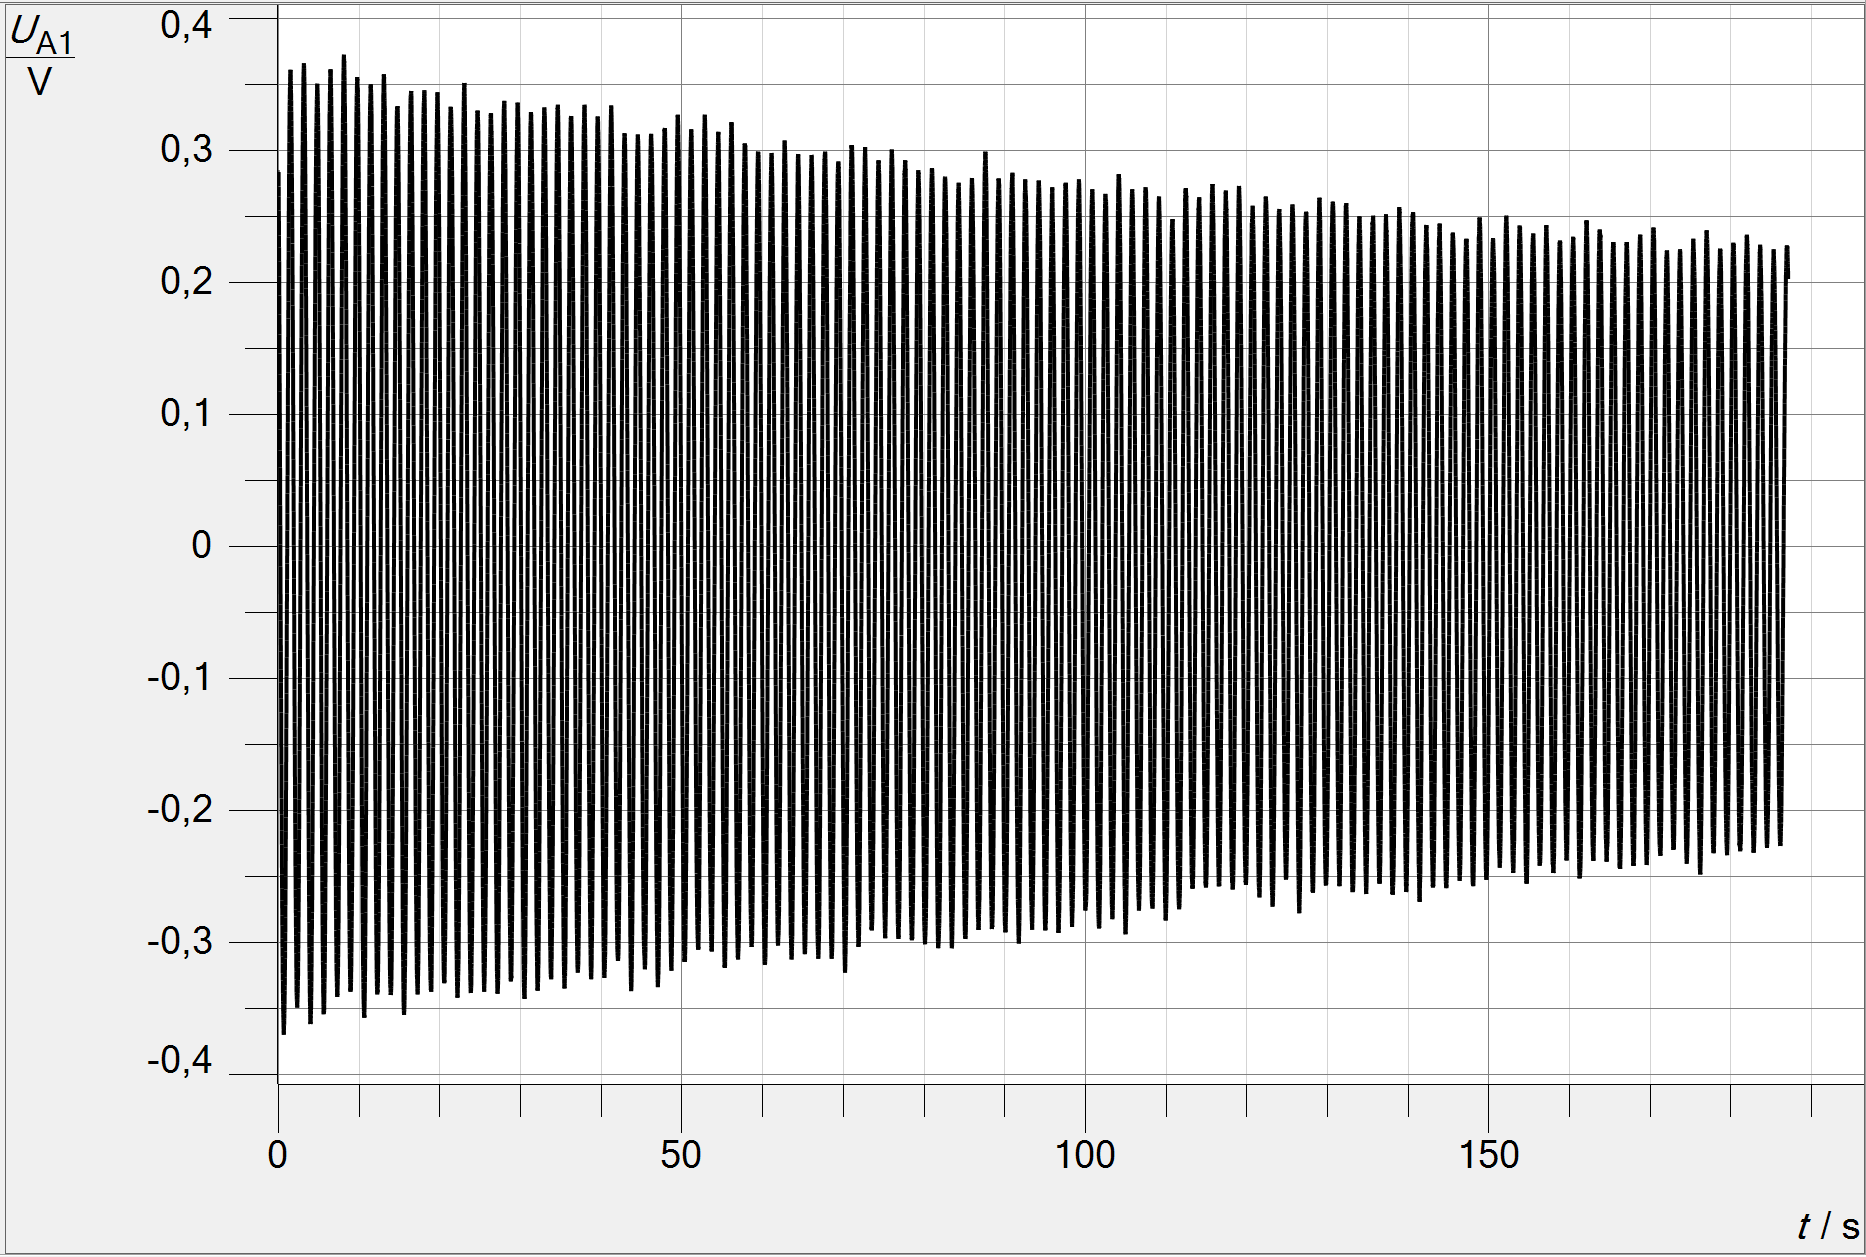
\includegraphics[width=0.9\textwidth]{plots/stange-1-komplett.PNG}
    \caption{Gesamtschwingungsverlauf der ersten Messung ohne Pendelkörper}
\end{figure}
Hier können sie Exemplarisch den Gesamtschwingungsverlauf der ersten Messung sehen bis 185 Sekunden.
Gut zu erkennen ist, dass wir eine Dämpfung der Schwingung haben.
Dies kann man daran sehen, dass die Amplitude der Schwingung mit der Zeit abnimmt. 

Um den genauen Verlauf der Schwingung nach zu volziehen, betrachten wir einen Ausschnitt dieser. 
\begin{figure}[H]
    \centering
    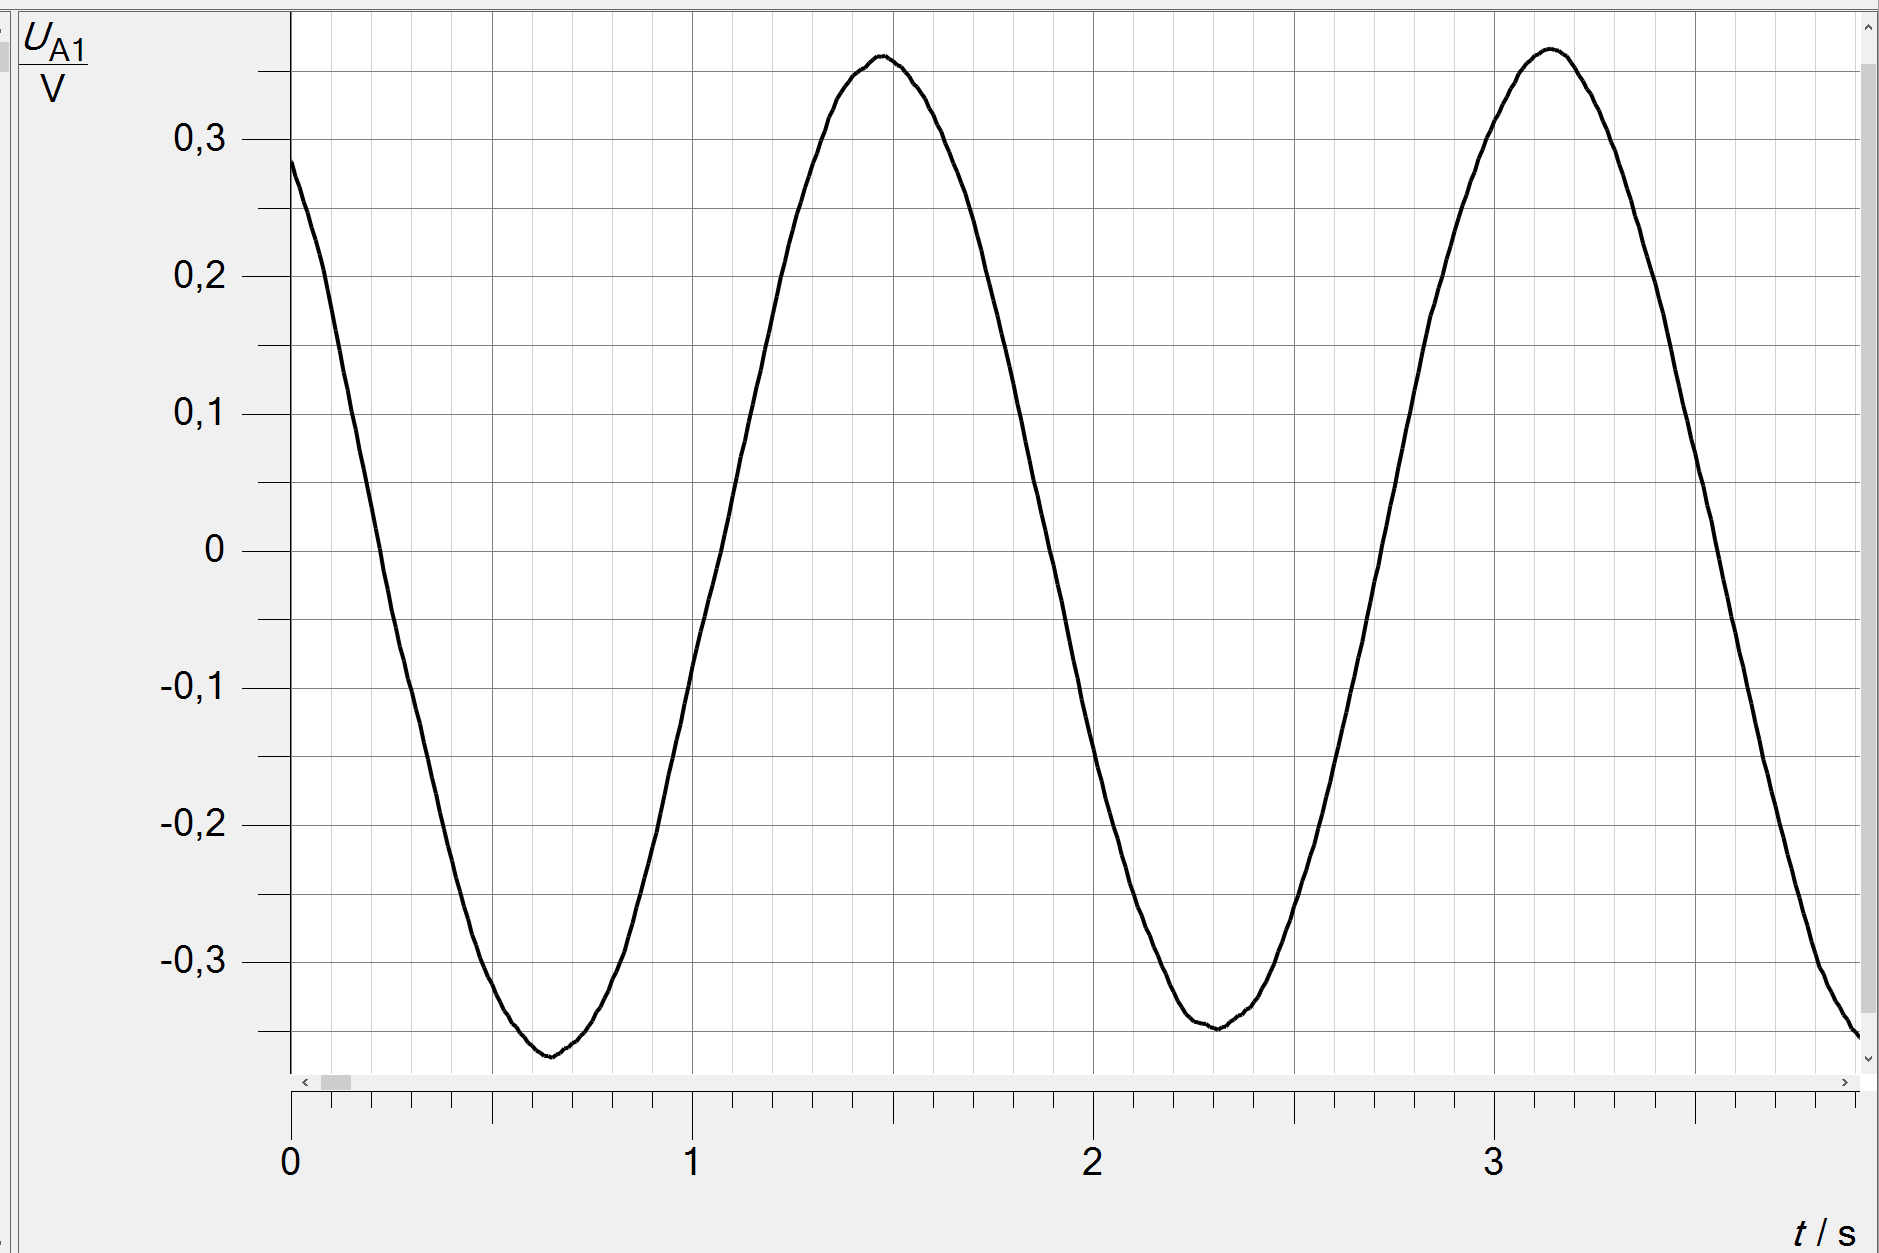
\includegraphics[width=0.7\textwidth]{plots/stange-1-mehrere-schwingungeng.PNG}
    \caption{Ausschnitt des Schwingungsverlauf der ersten Messung ohne Pendelkörper}
\end{figure}

Auf dem Bild sind die ersten 2.25 Schwingungsperioden zu sehen.
Hier können wir gut erkennen, dass die Schwingung einem Kosinus förmigen verlauf hat.  
Sie hat eine Amplitude von ca 0.35 Volt. 
Die in der Graphik angezeigte null Linie, wird nicht genau null sein, da es nicht möglich war den Winkelaufnehmer perfekt auf null zu kalibrieren.
Die leichten Unregelmäßigkeiten in der Kurve stammen daher, dass wir nur diskrete Messpunkte haben. 

\begin{figure}[H]
    \centering
    \subfloat{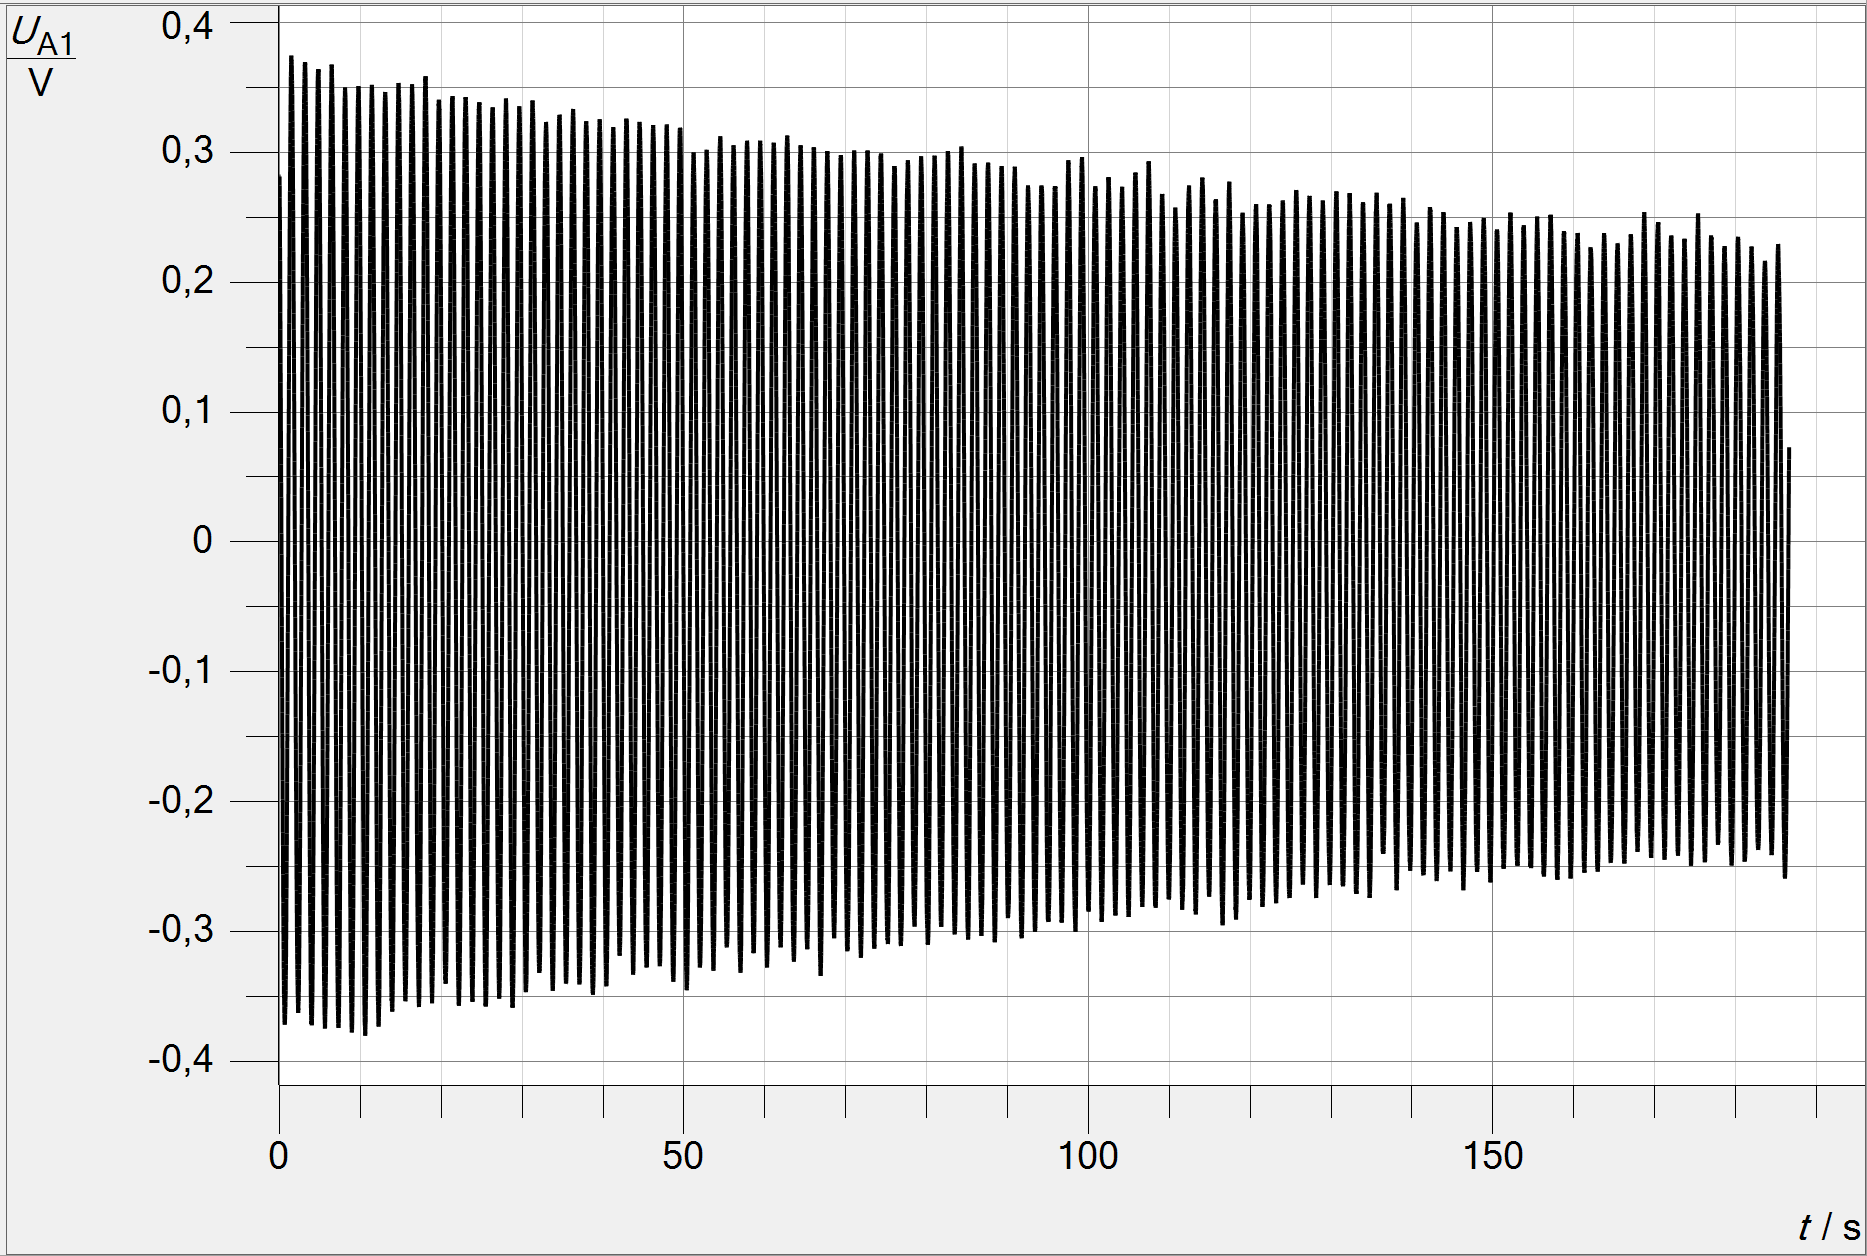
\includegraphics[width=0.45\textwidth]{plots/stange-2-komplett.PNG}}
    \hfill
    \subfloat{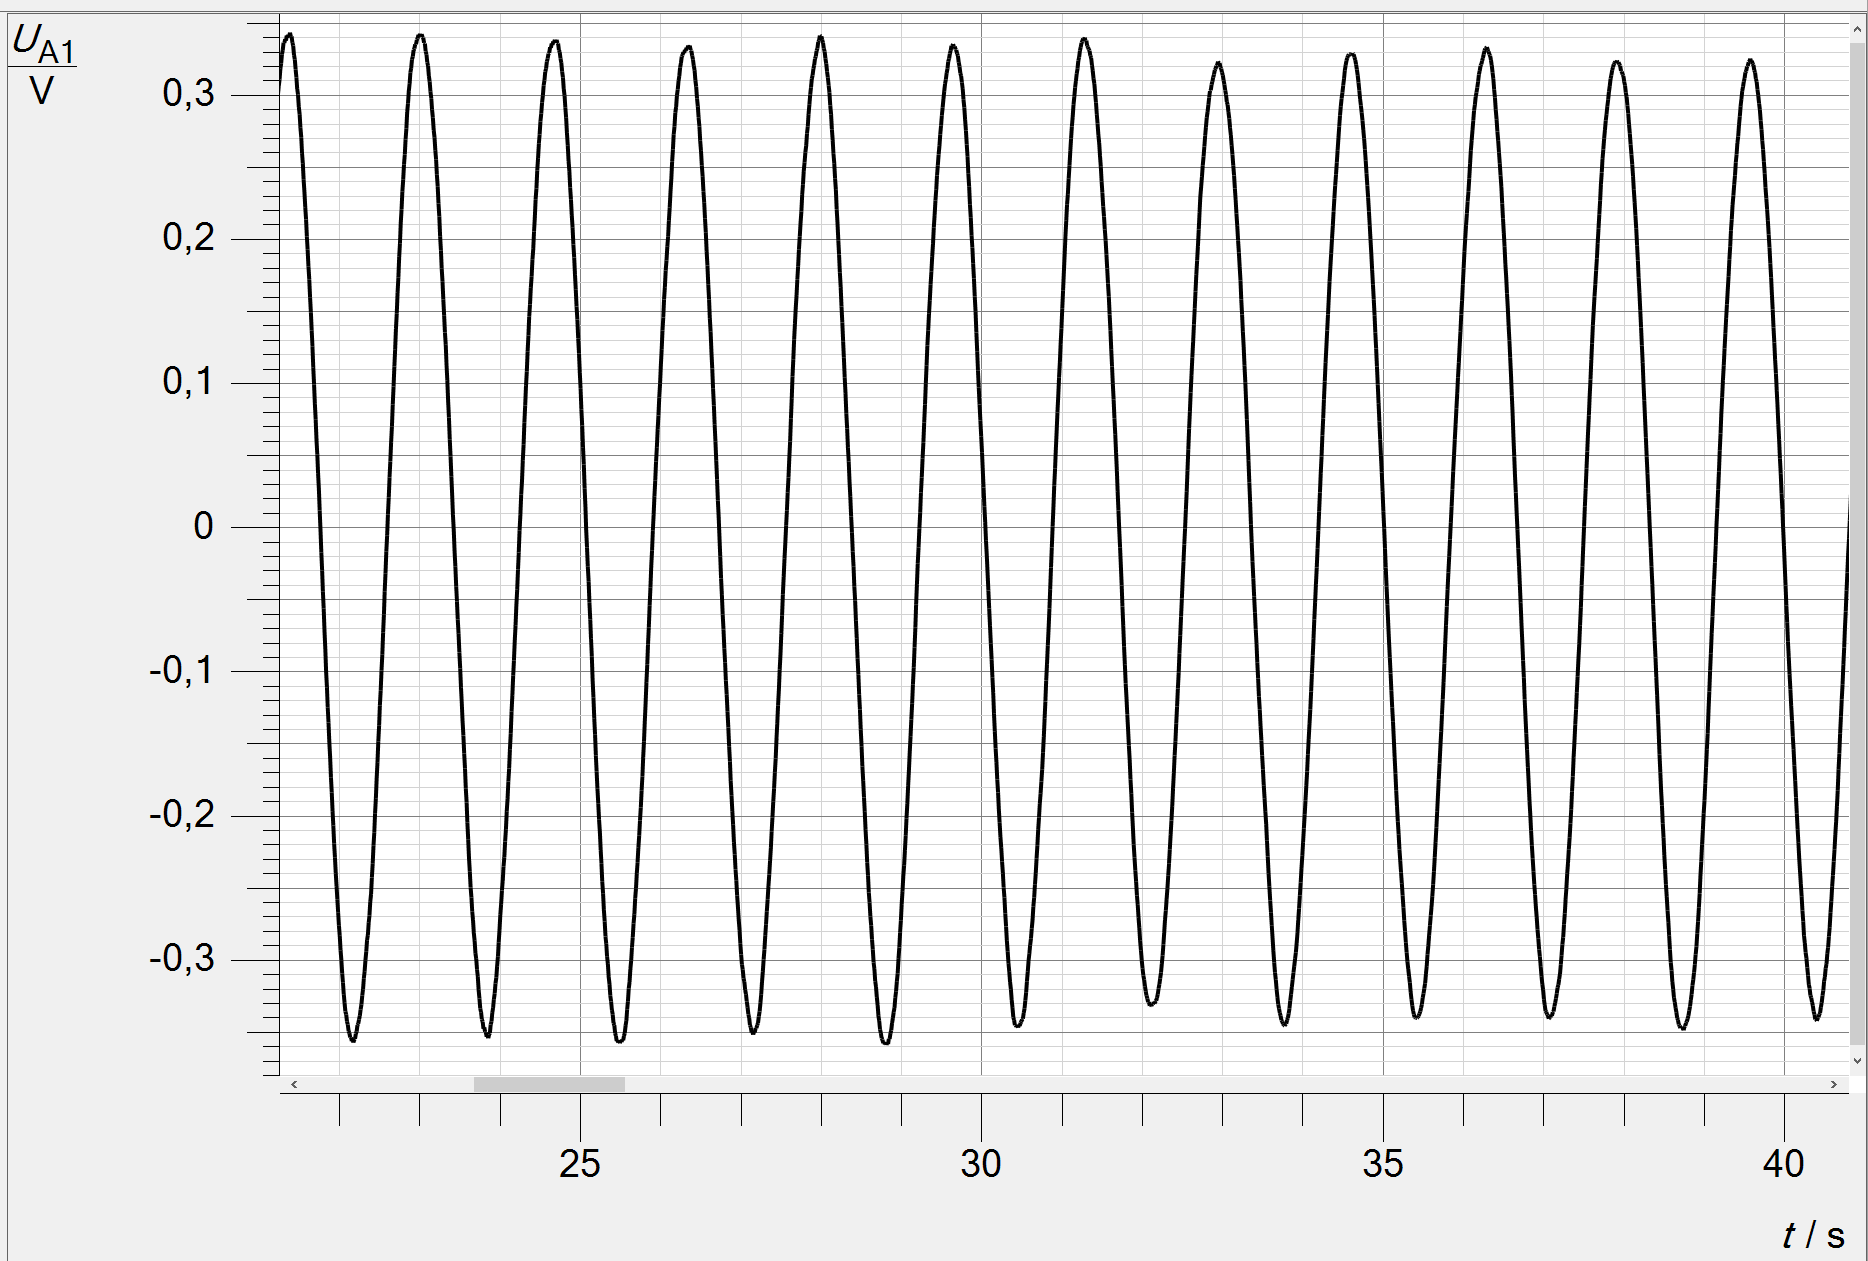
\includegraphics[width=0.45\textwidth]{plots/stange-2-mehrere-schwingungeng.PNG}}
    \caption{Schwingungsverläufe der zweiten Messung ohne Pendelkörper}
\end{figure}

Hier sind die Schwingungsverläufe der zweiten Messung ohne Pendelkörper dargestellt. 
Auch hier können wir die Abnahme der Amplitude sehen.
Hier ist ein größerer Ausschnitt zu sehen. Hier kann man erkennen, dass die Schwingung auch Kosinus förmig verläuft. 
Beim betrachten der Gesamten Schwingung in CASSY konnten wir sehen, dass dieser Kosinus förmige verlauf die gesamte Messung über beibehalten wird.
Dies stimmt auch mit den Theoretischen Erwartungen überein.

\begin{figure}[H]
    \centering
    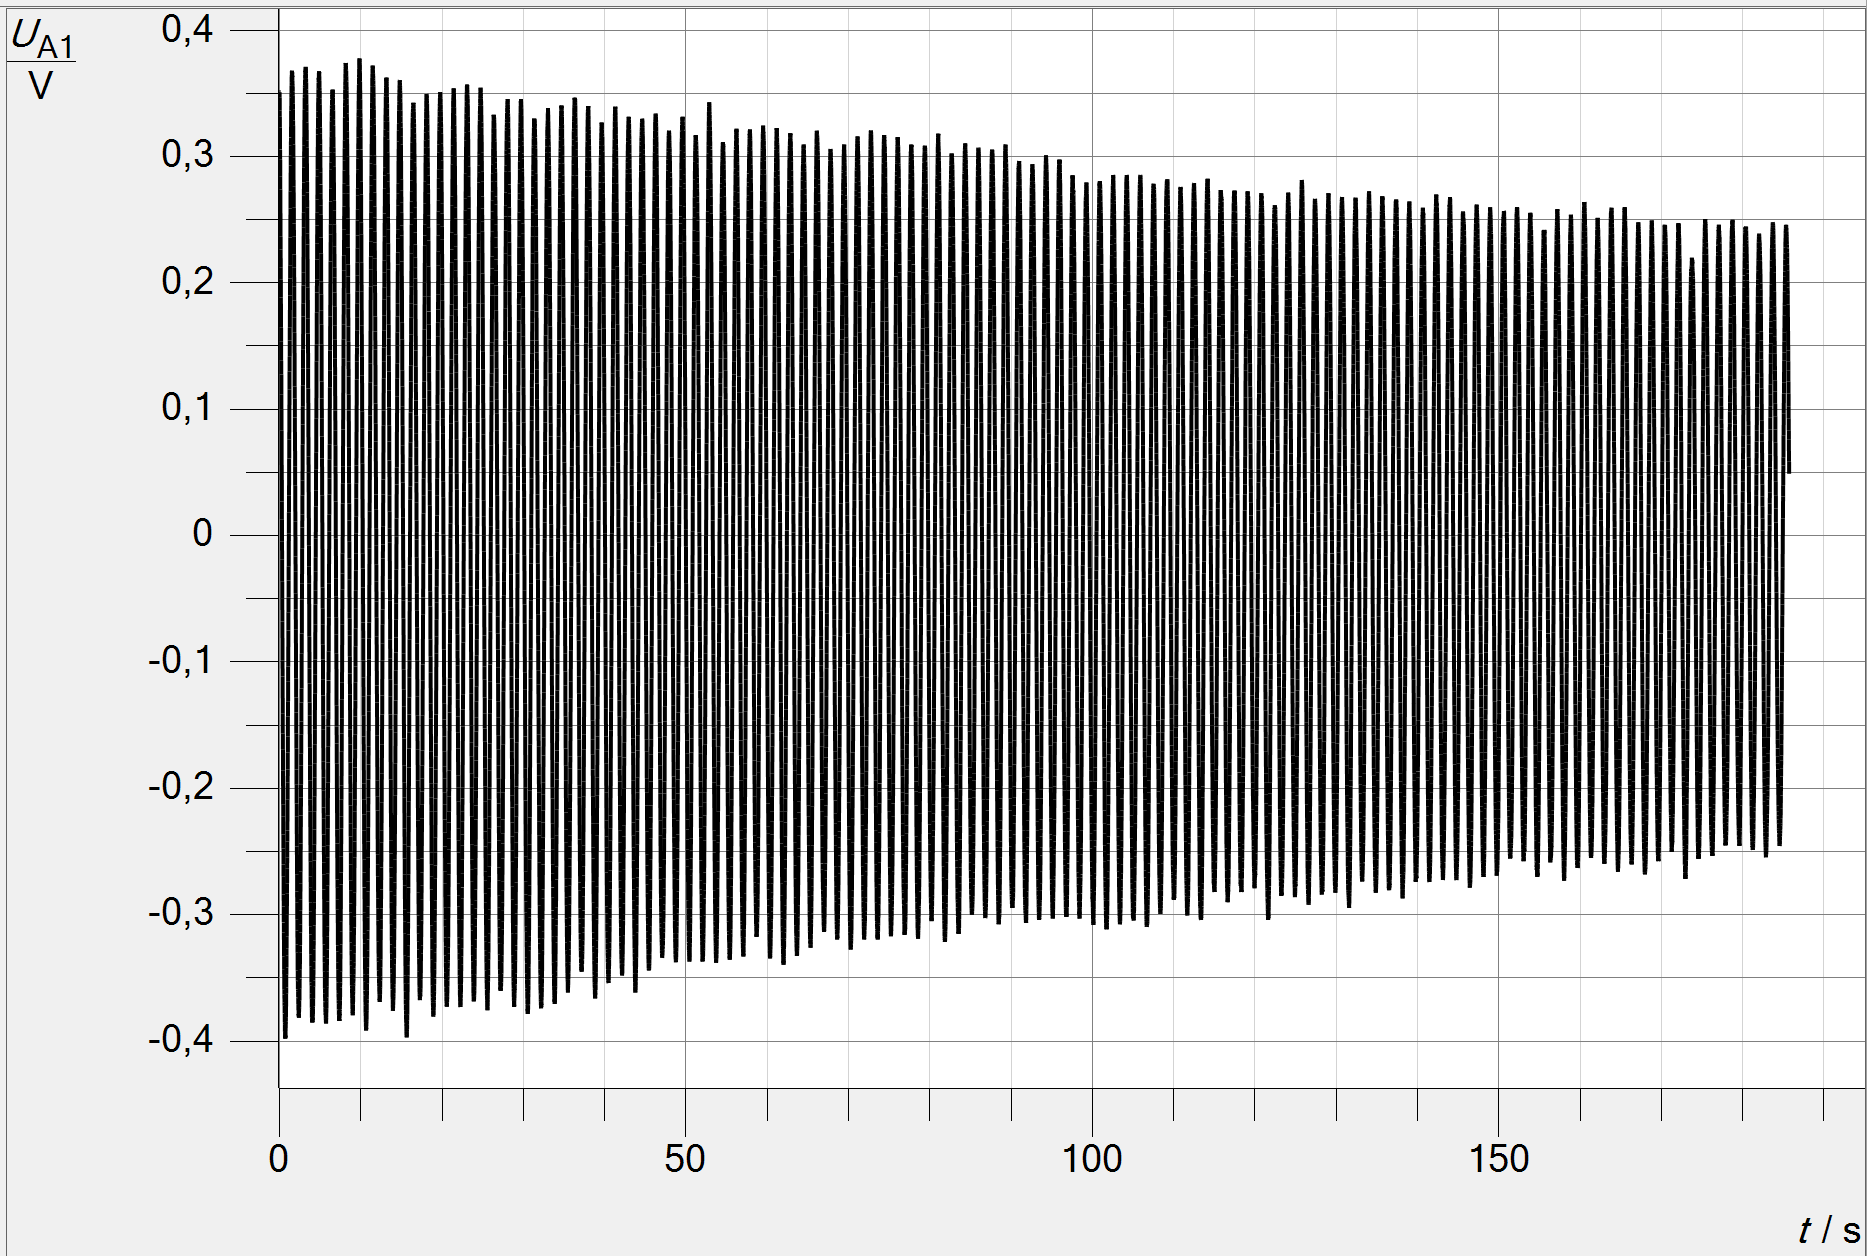
\includegraphics[width=0.7\textwidth]{plots/stange-3-komplett.PNG}
    \caption{Schwingungsverlauf der dritten Messung ohne Pendelkörper}
\end{figure}
\begin{figure}[H]
    \centering
    \subfloat{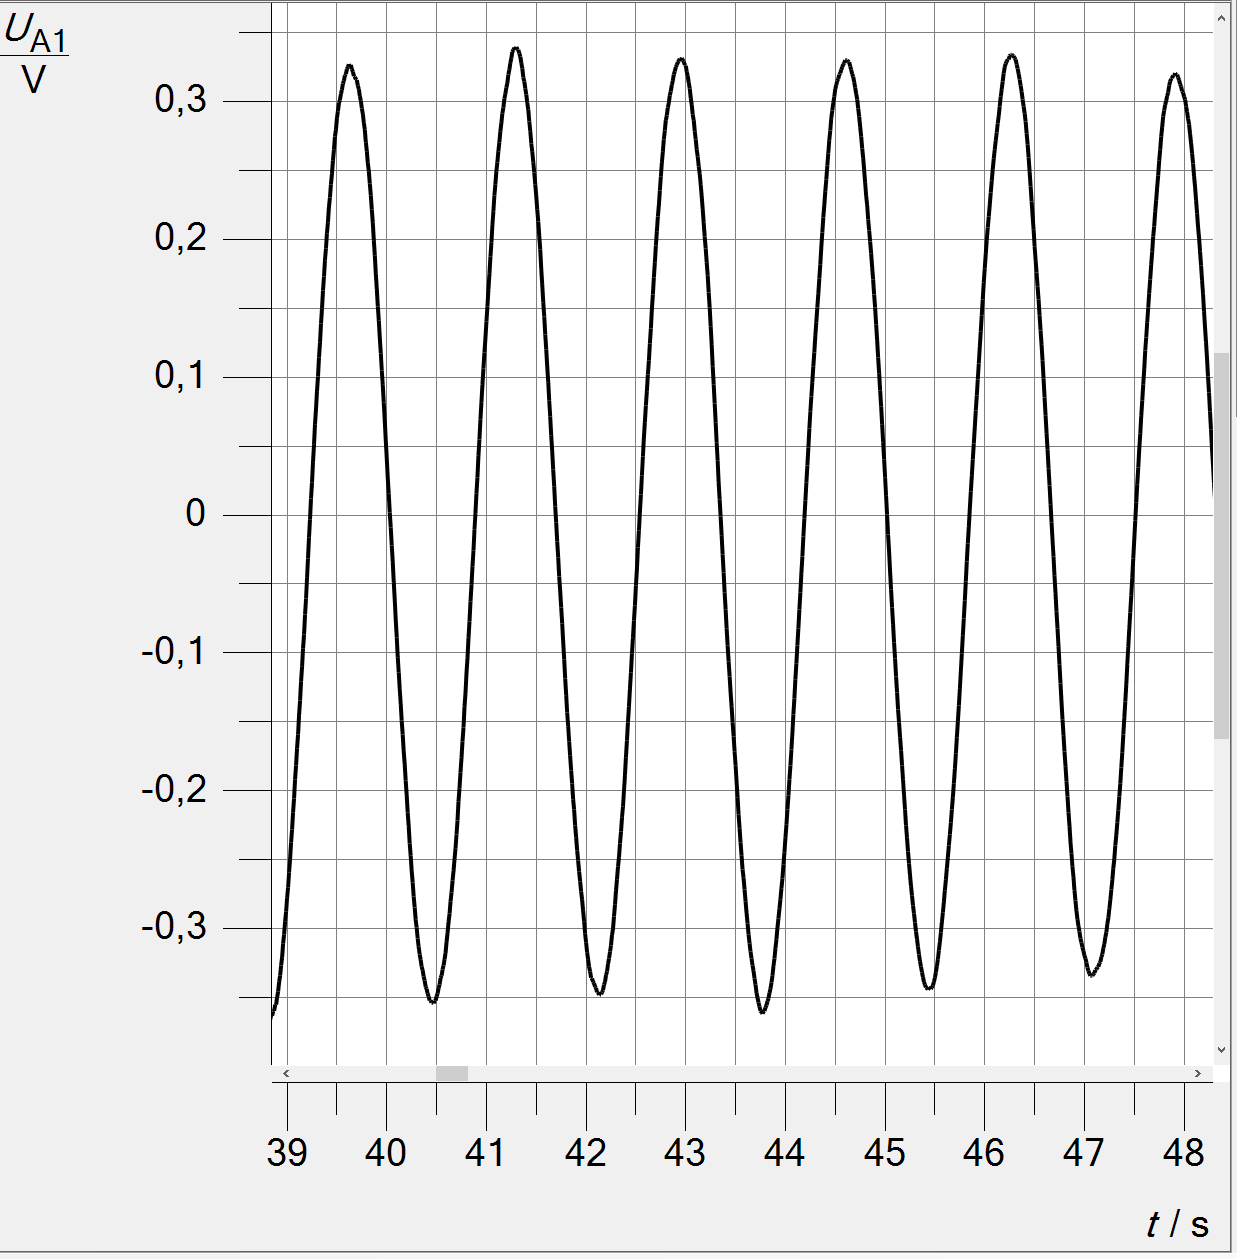
\includegraphics[width=0.45\textwidth]{plots/stange-3-mehrere-schwingungeng.PNG}}
    \hfill
    \subfloat{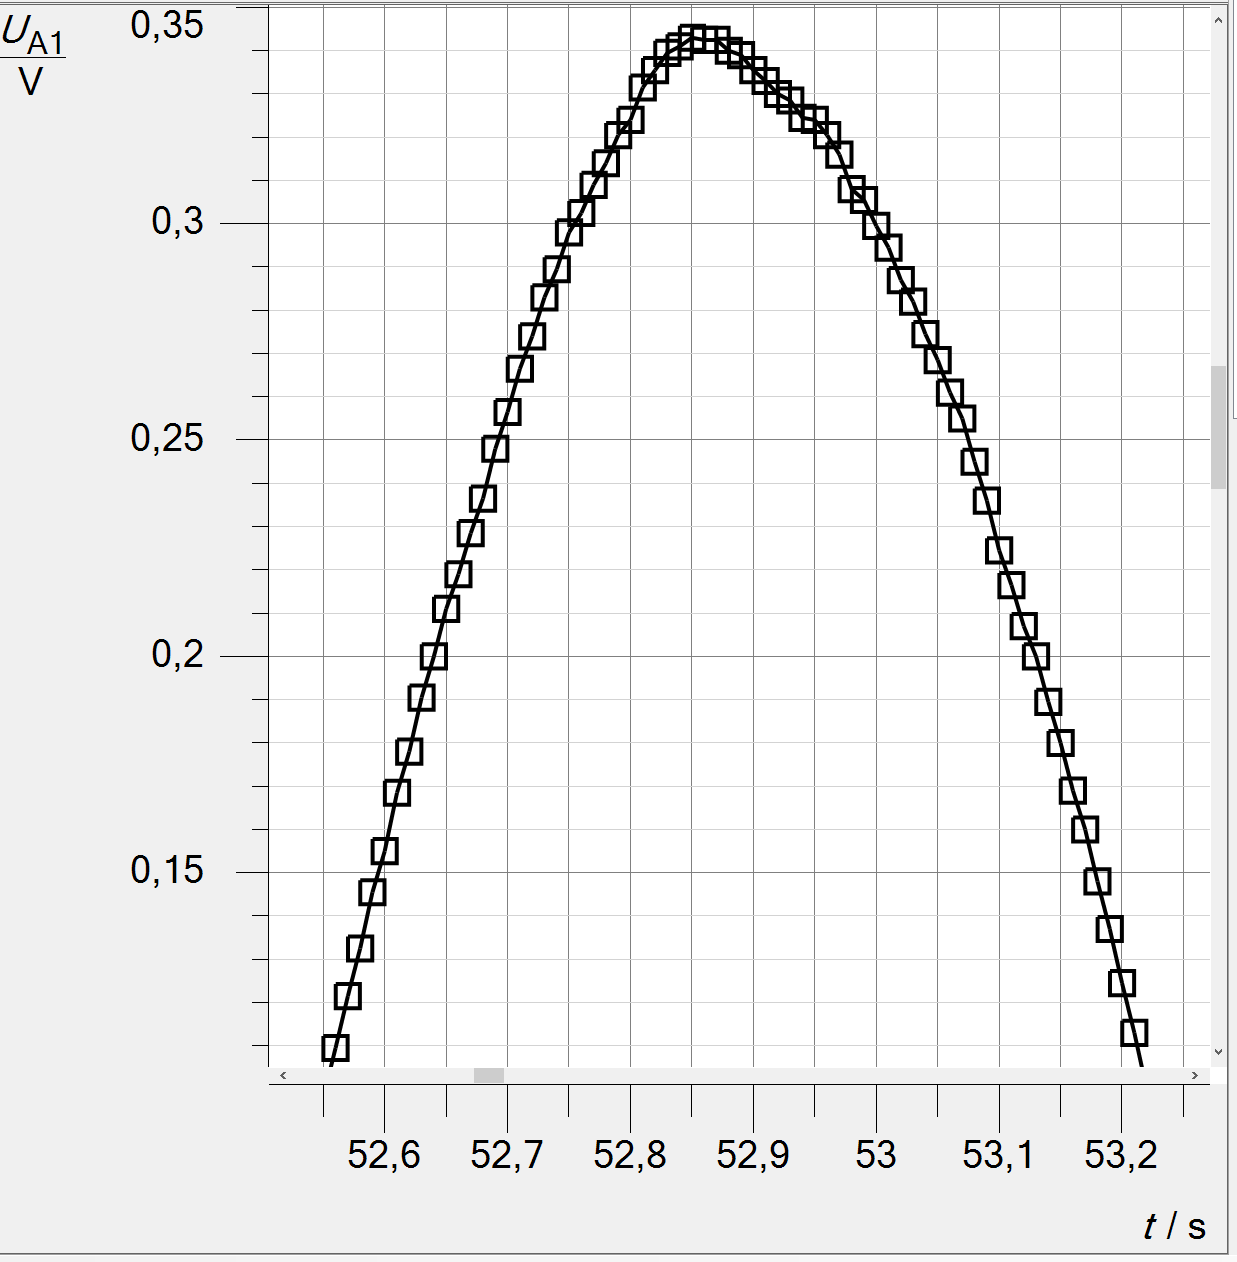
\includegraphics[width=0.45\textwidth]{plots/stange-3-maximum.PNG}}
    \caption{Ausschnitt des Schwingungsverlauf der dritten Messung ohne Pendelkörper}
\end{figure}

Hier sind die Schwingungsverläufe der dritten Messung dargestellt. Diese weisen die selbe Charakteristik auf wie die vorherigen.
Dieses Bild zeigt exemplarisch ein Maxima der Schwingung mit eingezeichneten Datenpunkten. 
Gut zu sehen ist, dass wir diskrete Datenpunkte haben, es liegen genug Datenpunkte im Bereich des Maximums um mit diesen das Maximum zu bestimmen.\\
%TODO : Einfügen eines Bilds wo der erste Peak bestimmt wird
Während den Messungen haben wir damit wir die Periodendauer überschlagen können, bei CASSY mit dem Peakschwerpunkt das erste und das zwanzigste Maximum bestimmt.

Sobald das Pendel mit Pendelkörper synchronisiert war zu dem ohne Pendelkörper haben wir hier auch drei Messungen durchgeführt.
\begin{figure}[H]
    \centering
    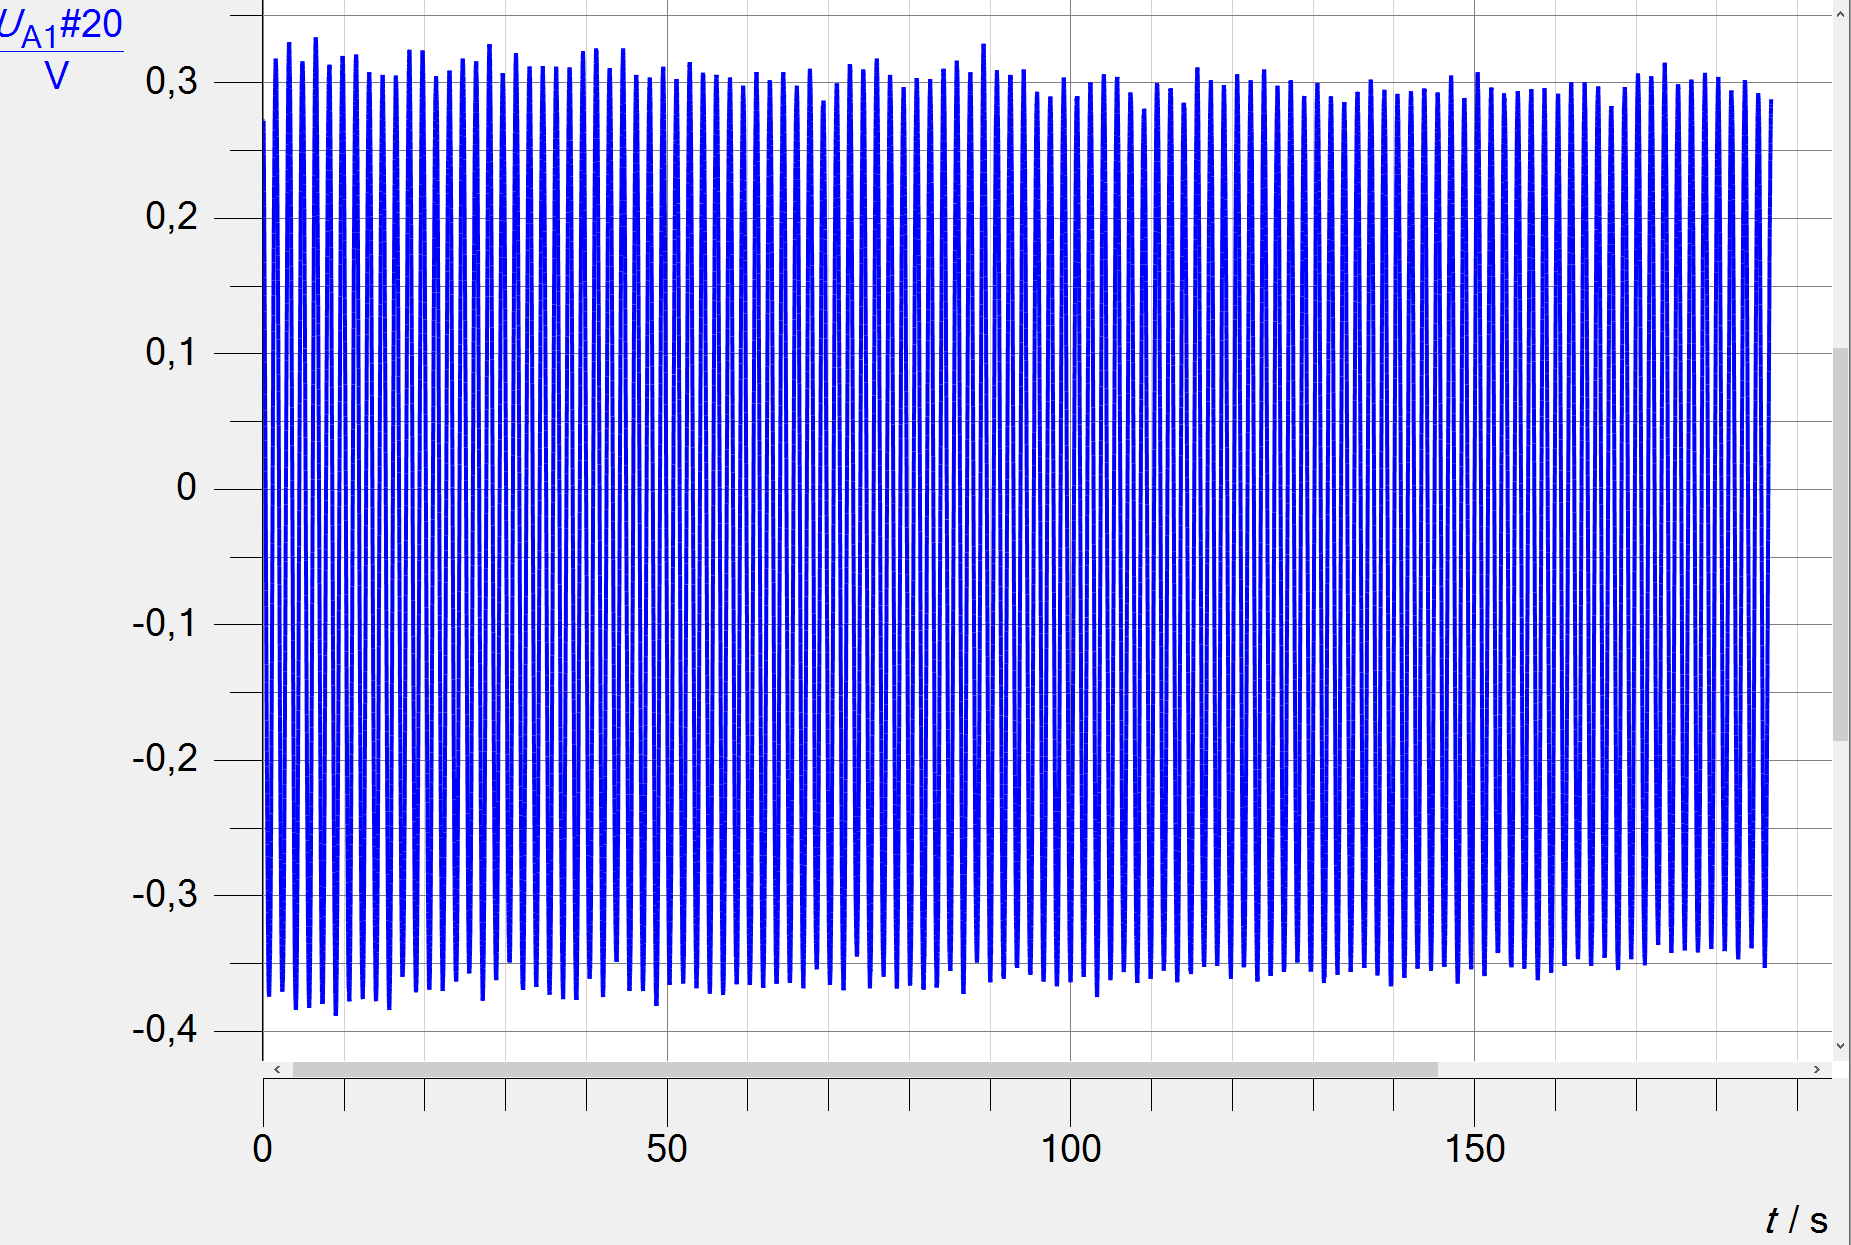
\includegraphics[width=0.9\textwidth]{plots/gewicht-1-komplett.PNG}
    \caption{Schwingungsverlauf der ersten Messung mit Pendelkörper}
    \end{figure}

In diesem Graphen kann man erkennen, dass im Gegensatz, zu dem Schwingvorgang ohne Pendelkörper, die Amplitude der Schwingung nicht abnimmt.
Die Dämpfung ist nach 185s also noch nicht zu sehen.\\

Die zwei Hauptfaktoren der Dämpfung sind der Luftwiederstand und die Reibung am Auflagepunkt der Nadel. 
Da wir keine Amplitudenabnahme mit Pendelkörper feststellen können, können wir daraus schließen, dass der Luftwiederstand den größeren Anteil der Dämpfung liefert.

\begin{figure}[H]
    \centering
    \subfloat{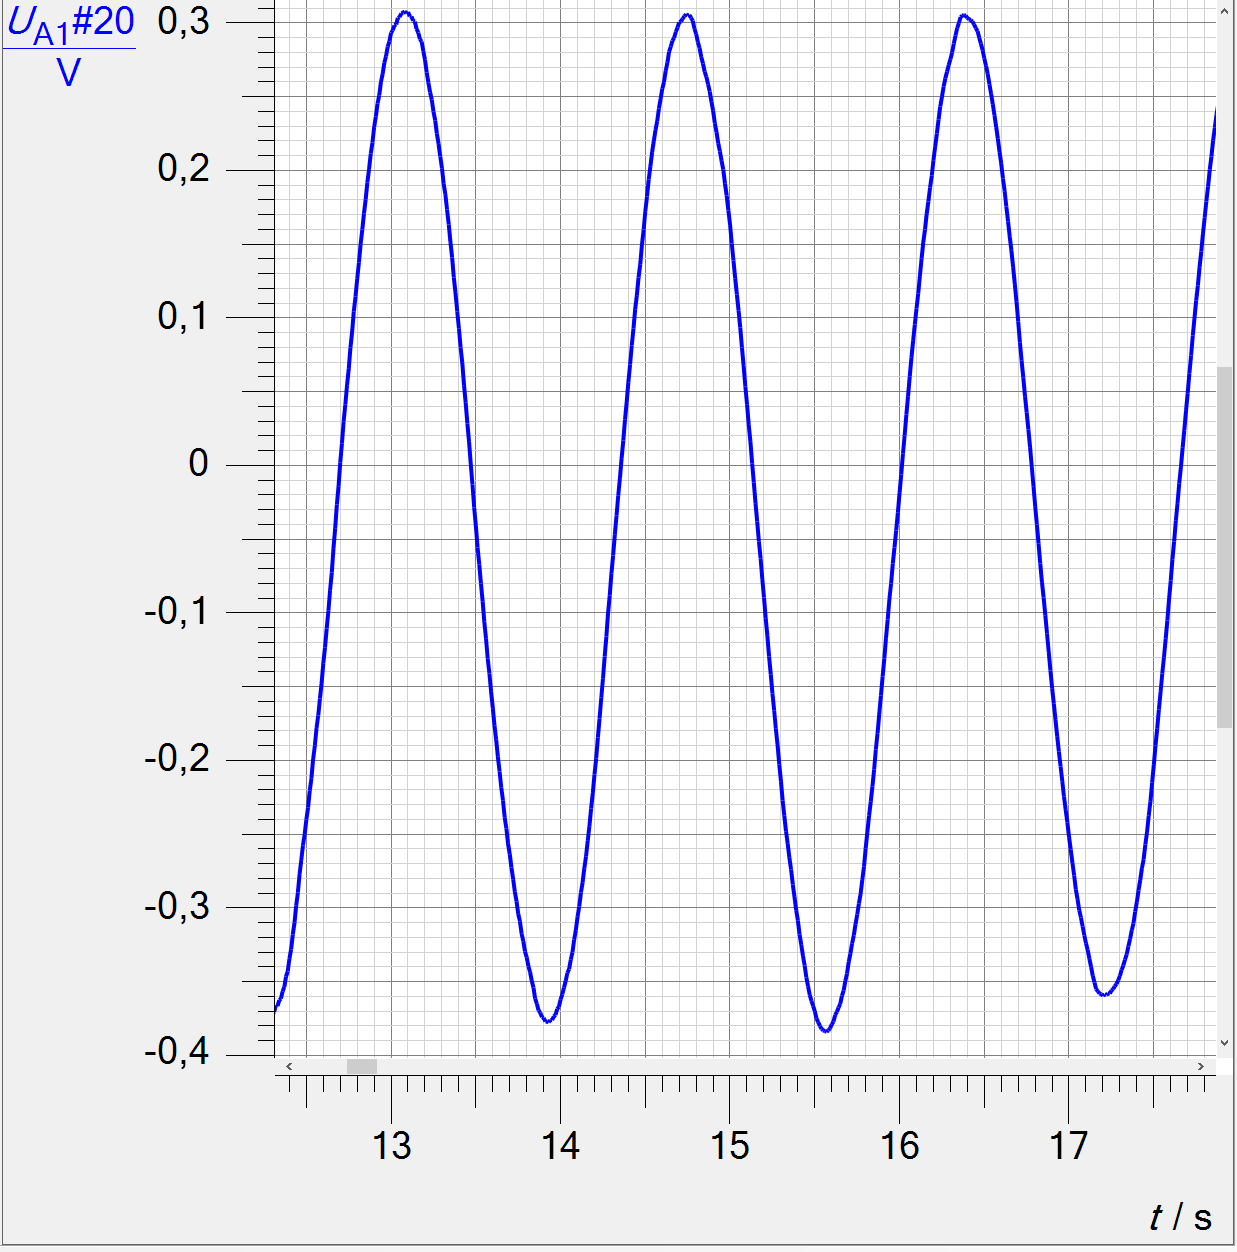
\includegraphics[width=0.4\textwidth]{plots/gewicht-1-mehrere-schwingungen.PNG}}
    \hfill
    \subfloat{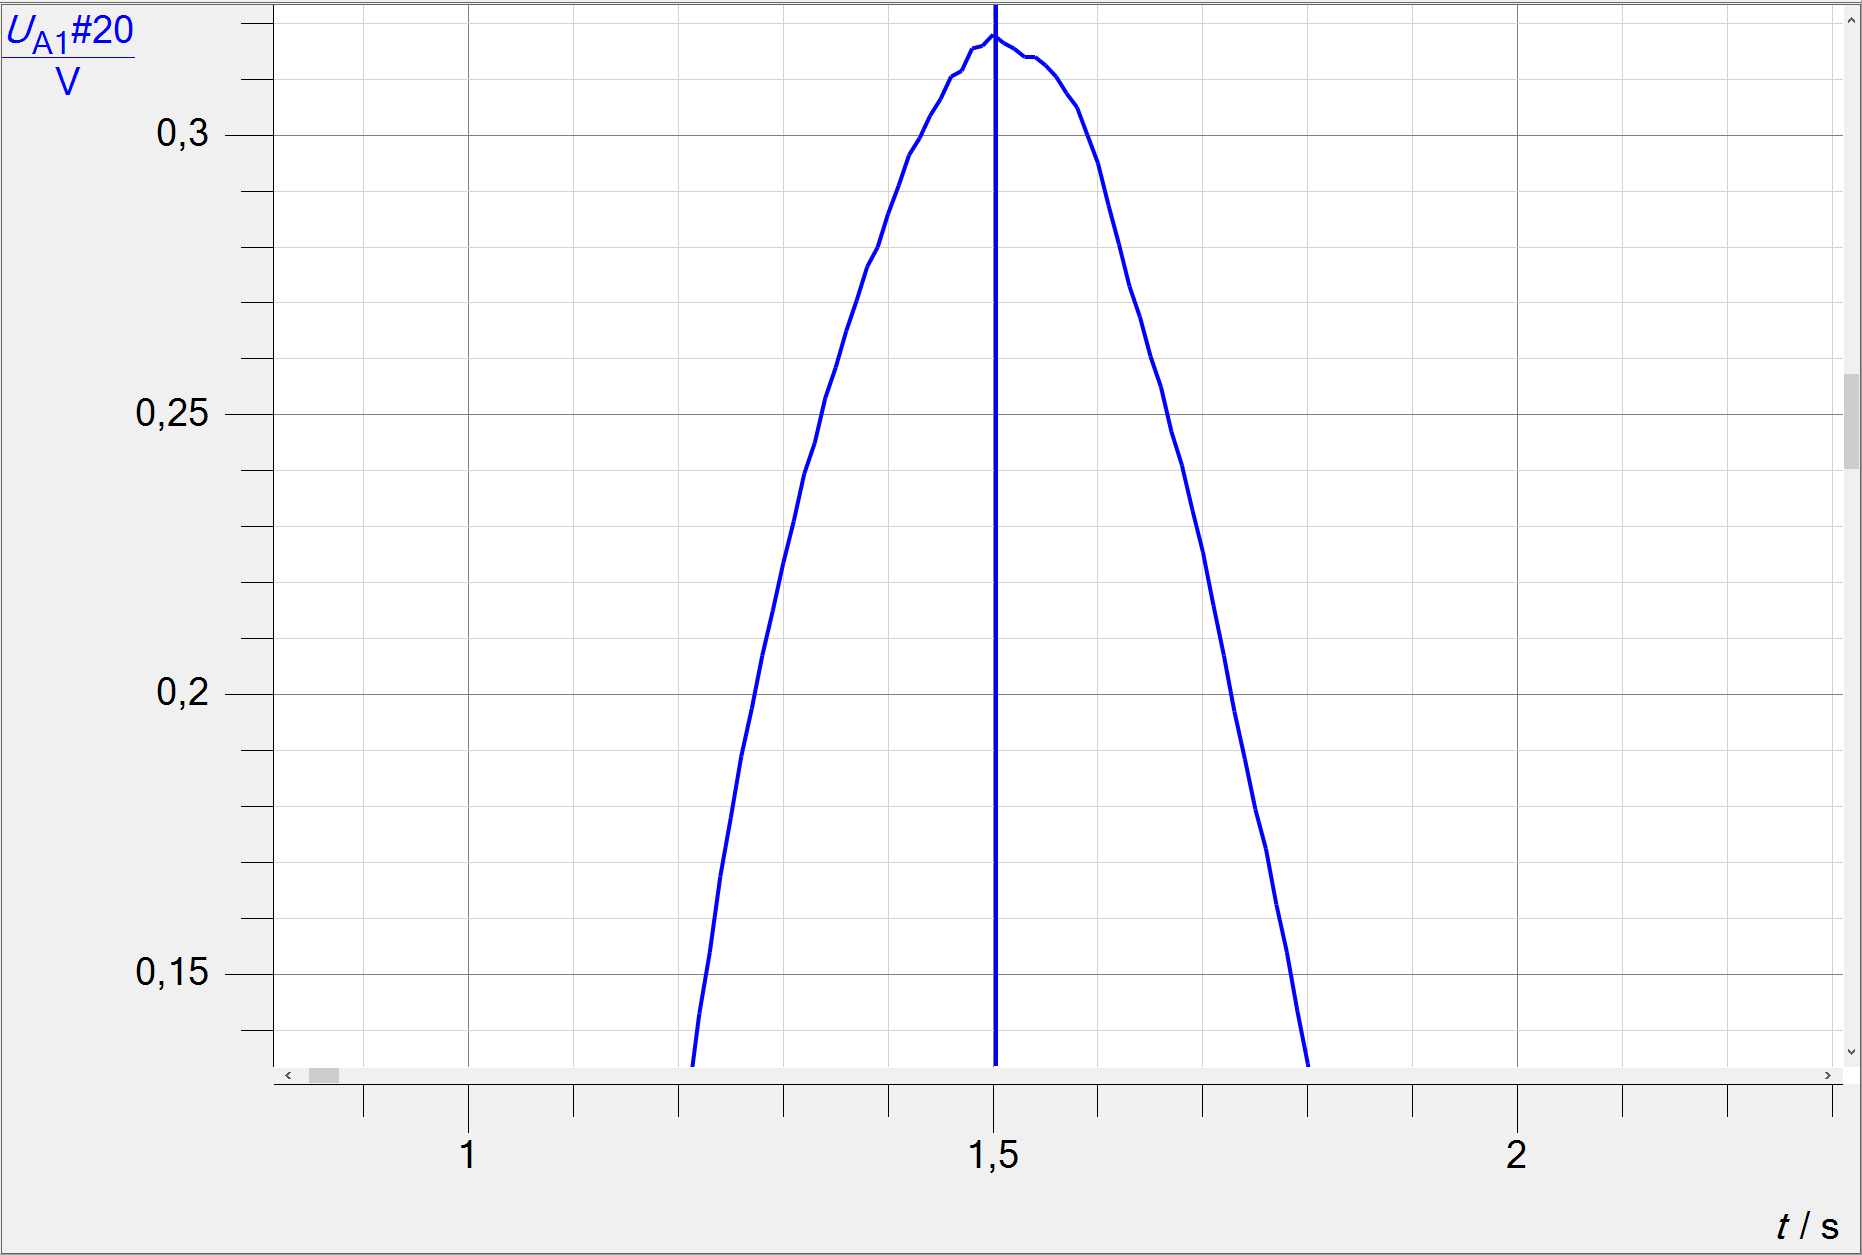
\includegraphics[width=0.55\textwidth]{plots/gewicht-1-peak-schnell.PNG}}
    \caption{Ausschnitt des Schwingungsverlauf der ersten Messung mit Pendelkörper}
    \end{figure}

Auch hier können wir erkennen, dass die Schwingung einem Kosinus förmigen Verlauf folgt.
Zum Vergleich der Periodendauern haben wir wieder das erste und das zwanzigste Maximum bestimmt.
Exemplarisch ist hier das Ablesen des ersten Maximums dargestellt.

Für die Weiteren Messungen sind hier auch die Schwingungsverläufe Dargestellt.
Für jede Messung der komplette Schwingungsverlauf und ein Ausschnitt der Schwingung. 

\begin{figure}[H]
    \centering
    \subfloat{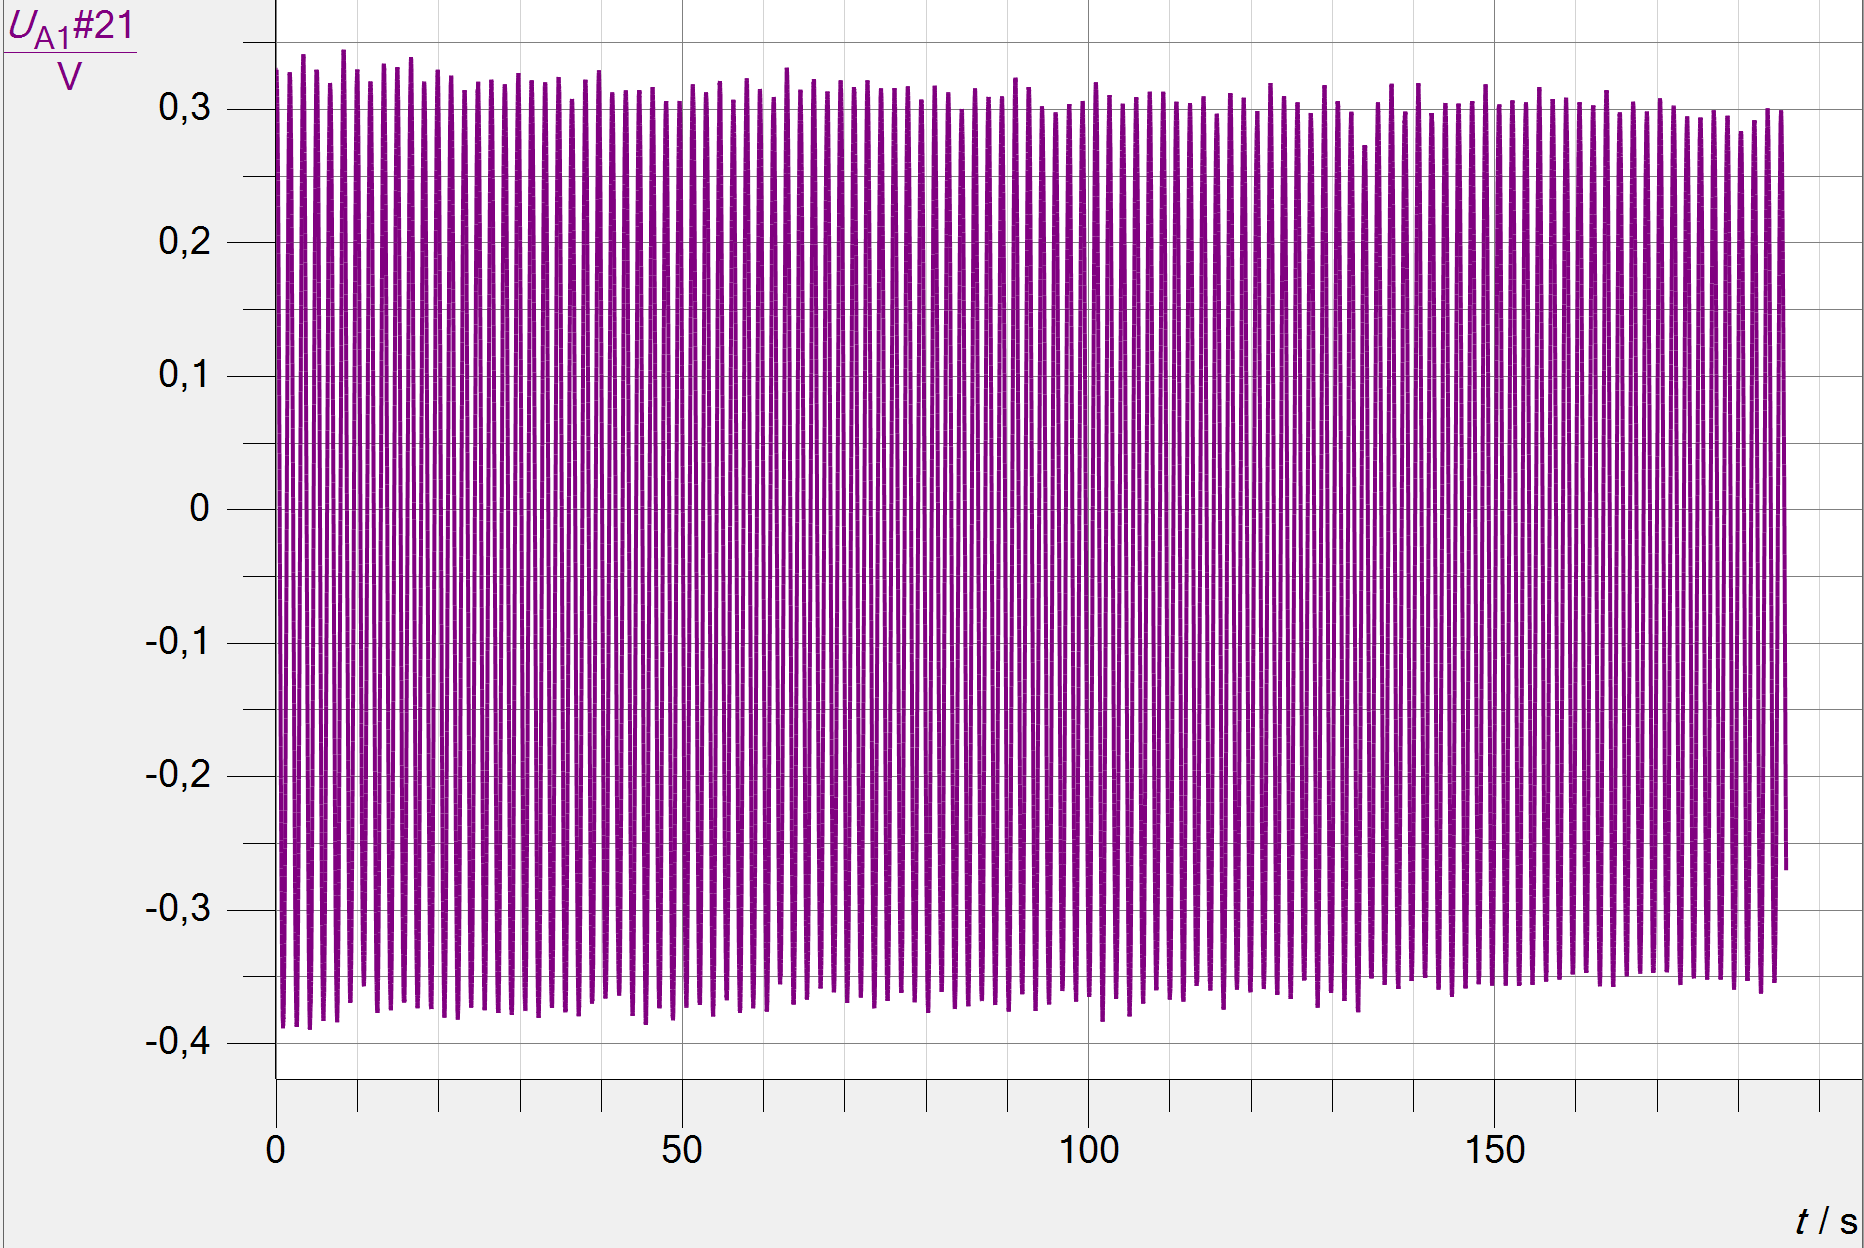
\includegraphics[width=0.55\textwidth]{plots/gewicht-2-komplett.PNG}}
    \hfill
    \subfloat{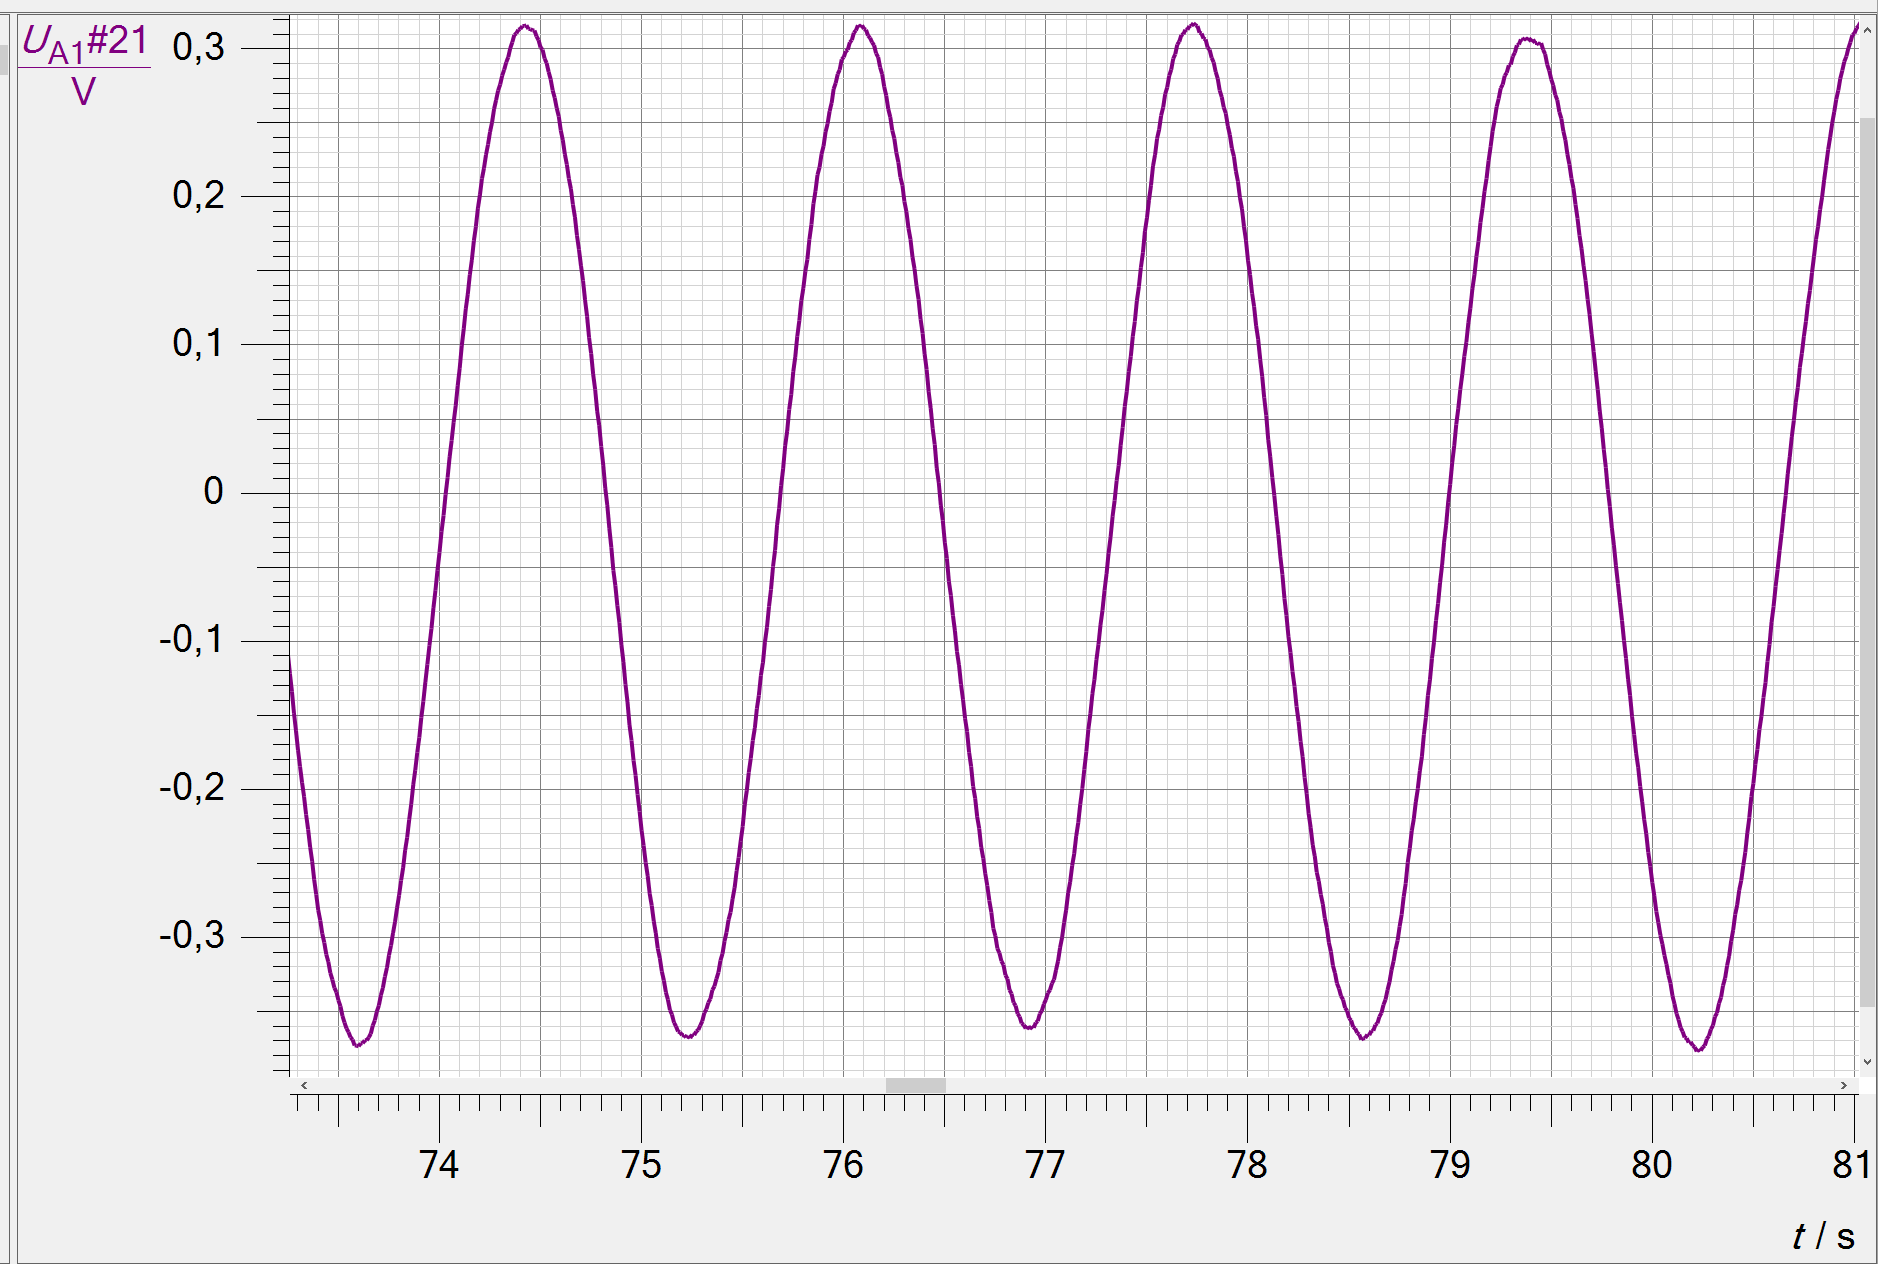
\includegraphics[width=0.40\textwidth]{plots/gewicht-2-schwungungen.PNG}}
    \caption{Schwingungsverlauf der zweiten Messung mit Pendelkörper}
    \end{figure}
 
\begin{figure}[H]
    \centering
    \subfloat{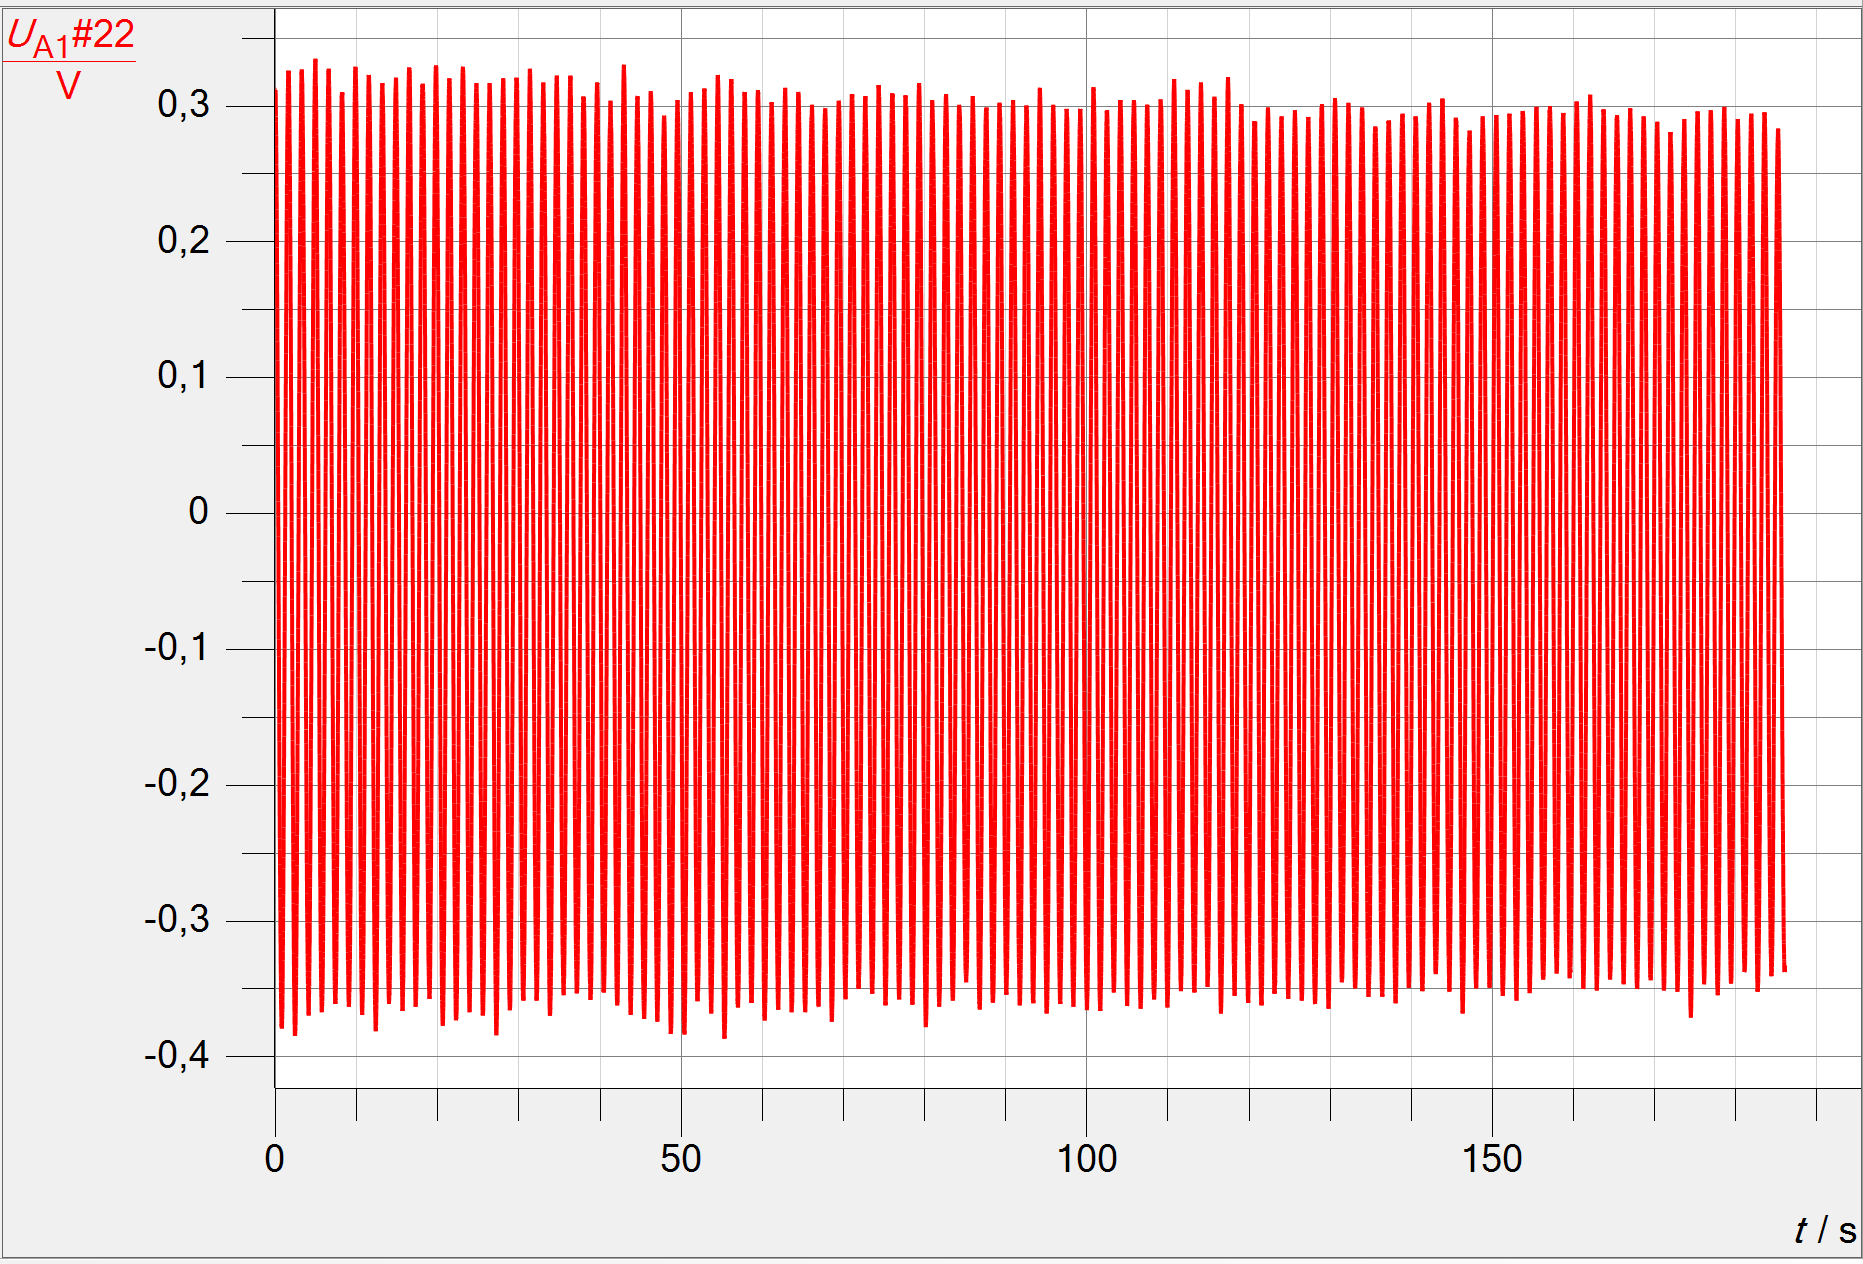
\includegraphics[width=0.55\textwidth]{plots/gewicht-3-komplett.PNG}}
    \hfill
    \subfloat{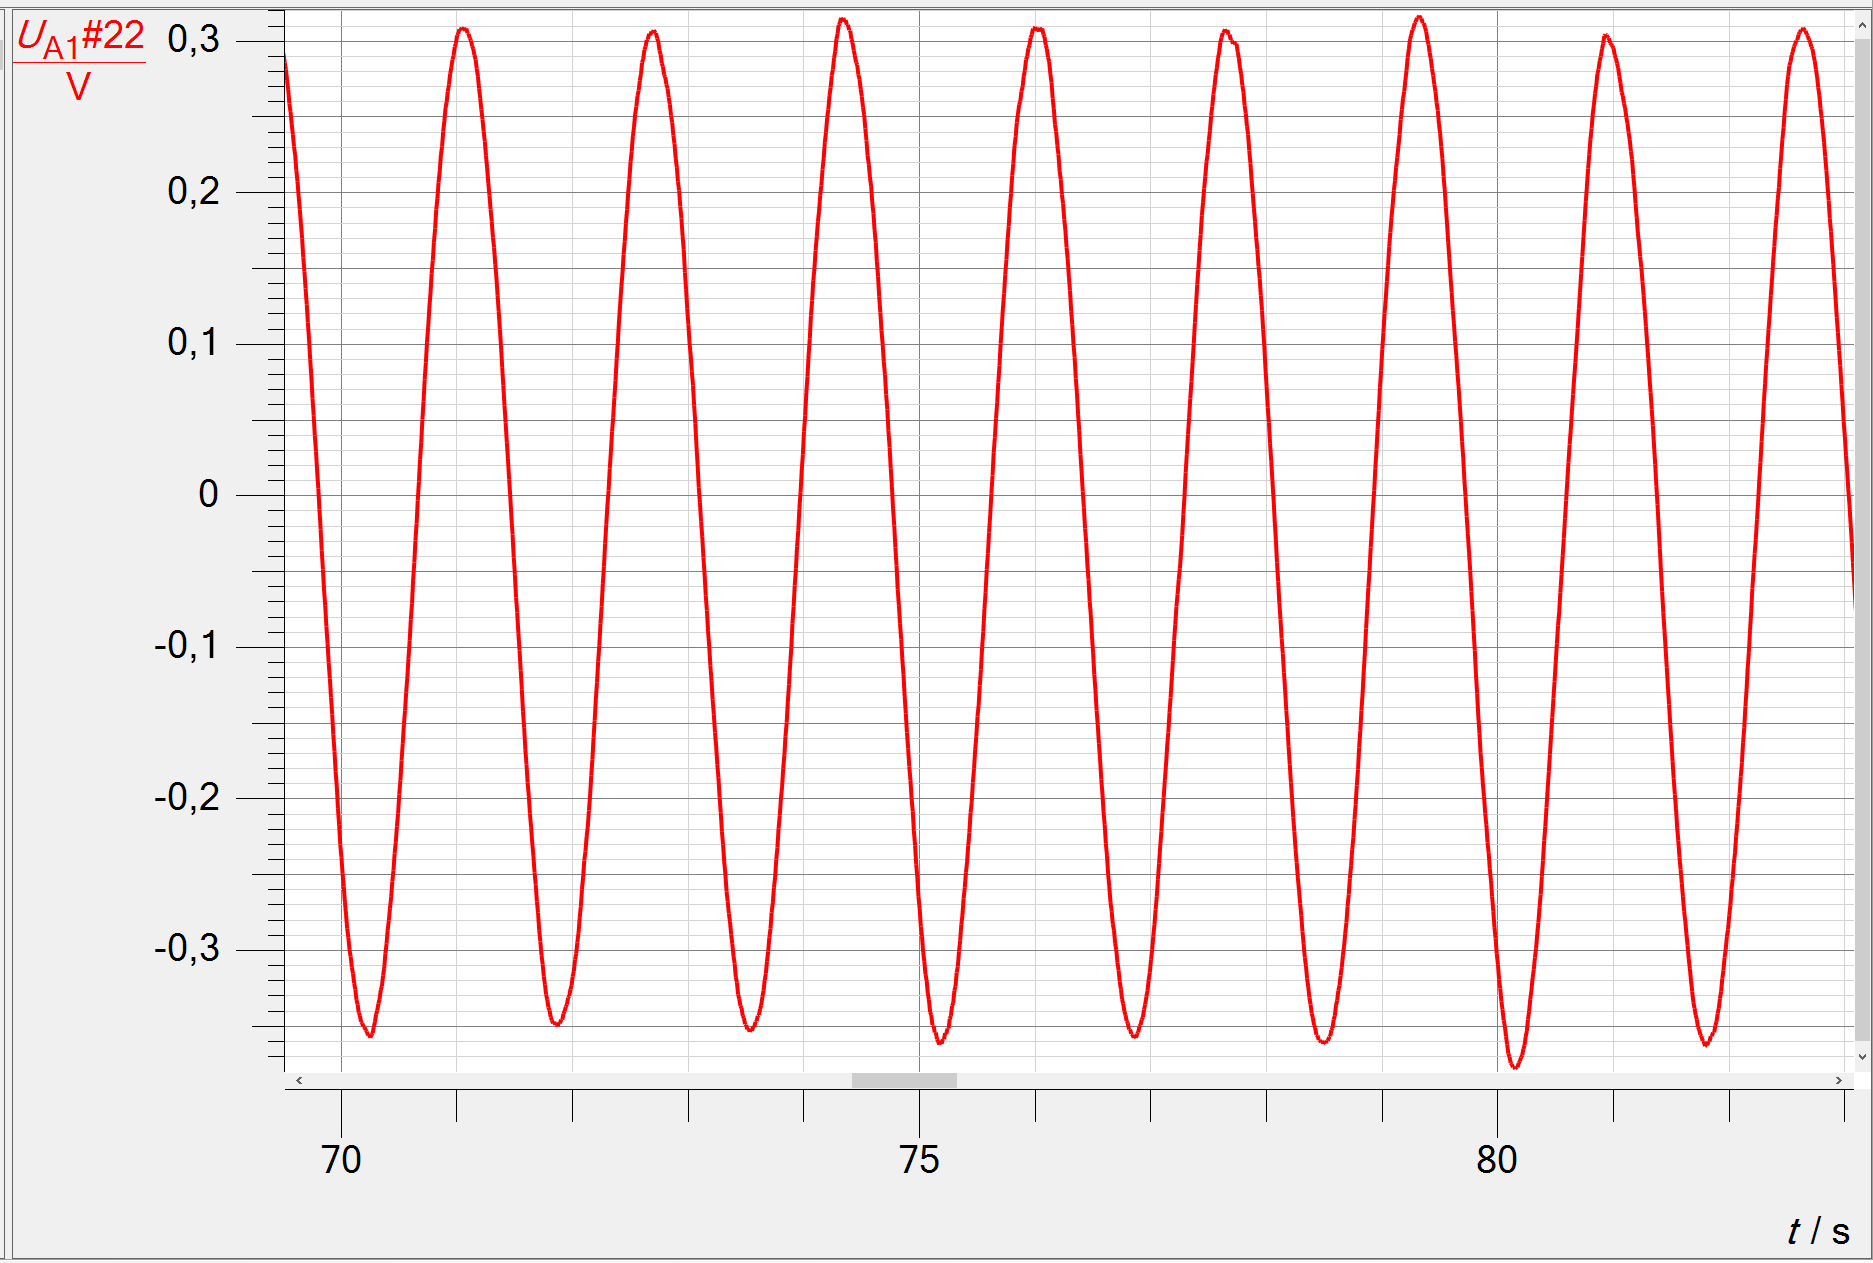
\includegraphics[width=0.40\textwidth]{plots/gewicht-3-schwungungen.PNG}}
    \caption{Schwingungsverlauf der dritten Messung mit Pendelkörper}
    \end{figure}

Zuletzt ist hier noch eine Nahaufnahme eines Maxima gezeigt, in dieser kann man erkennen, dass die Messpunkte um das Maxima nicht perfekt Kosinuns förmig sind.
Dies ist jedoch zur Bestimmung des Peaks kein problem, da wir hierfür den Peakschwerpunkt berechnen.

\begin{figure}[H]
    \centering
    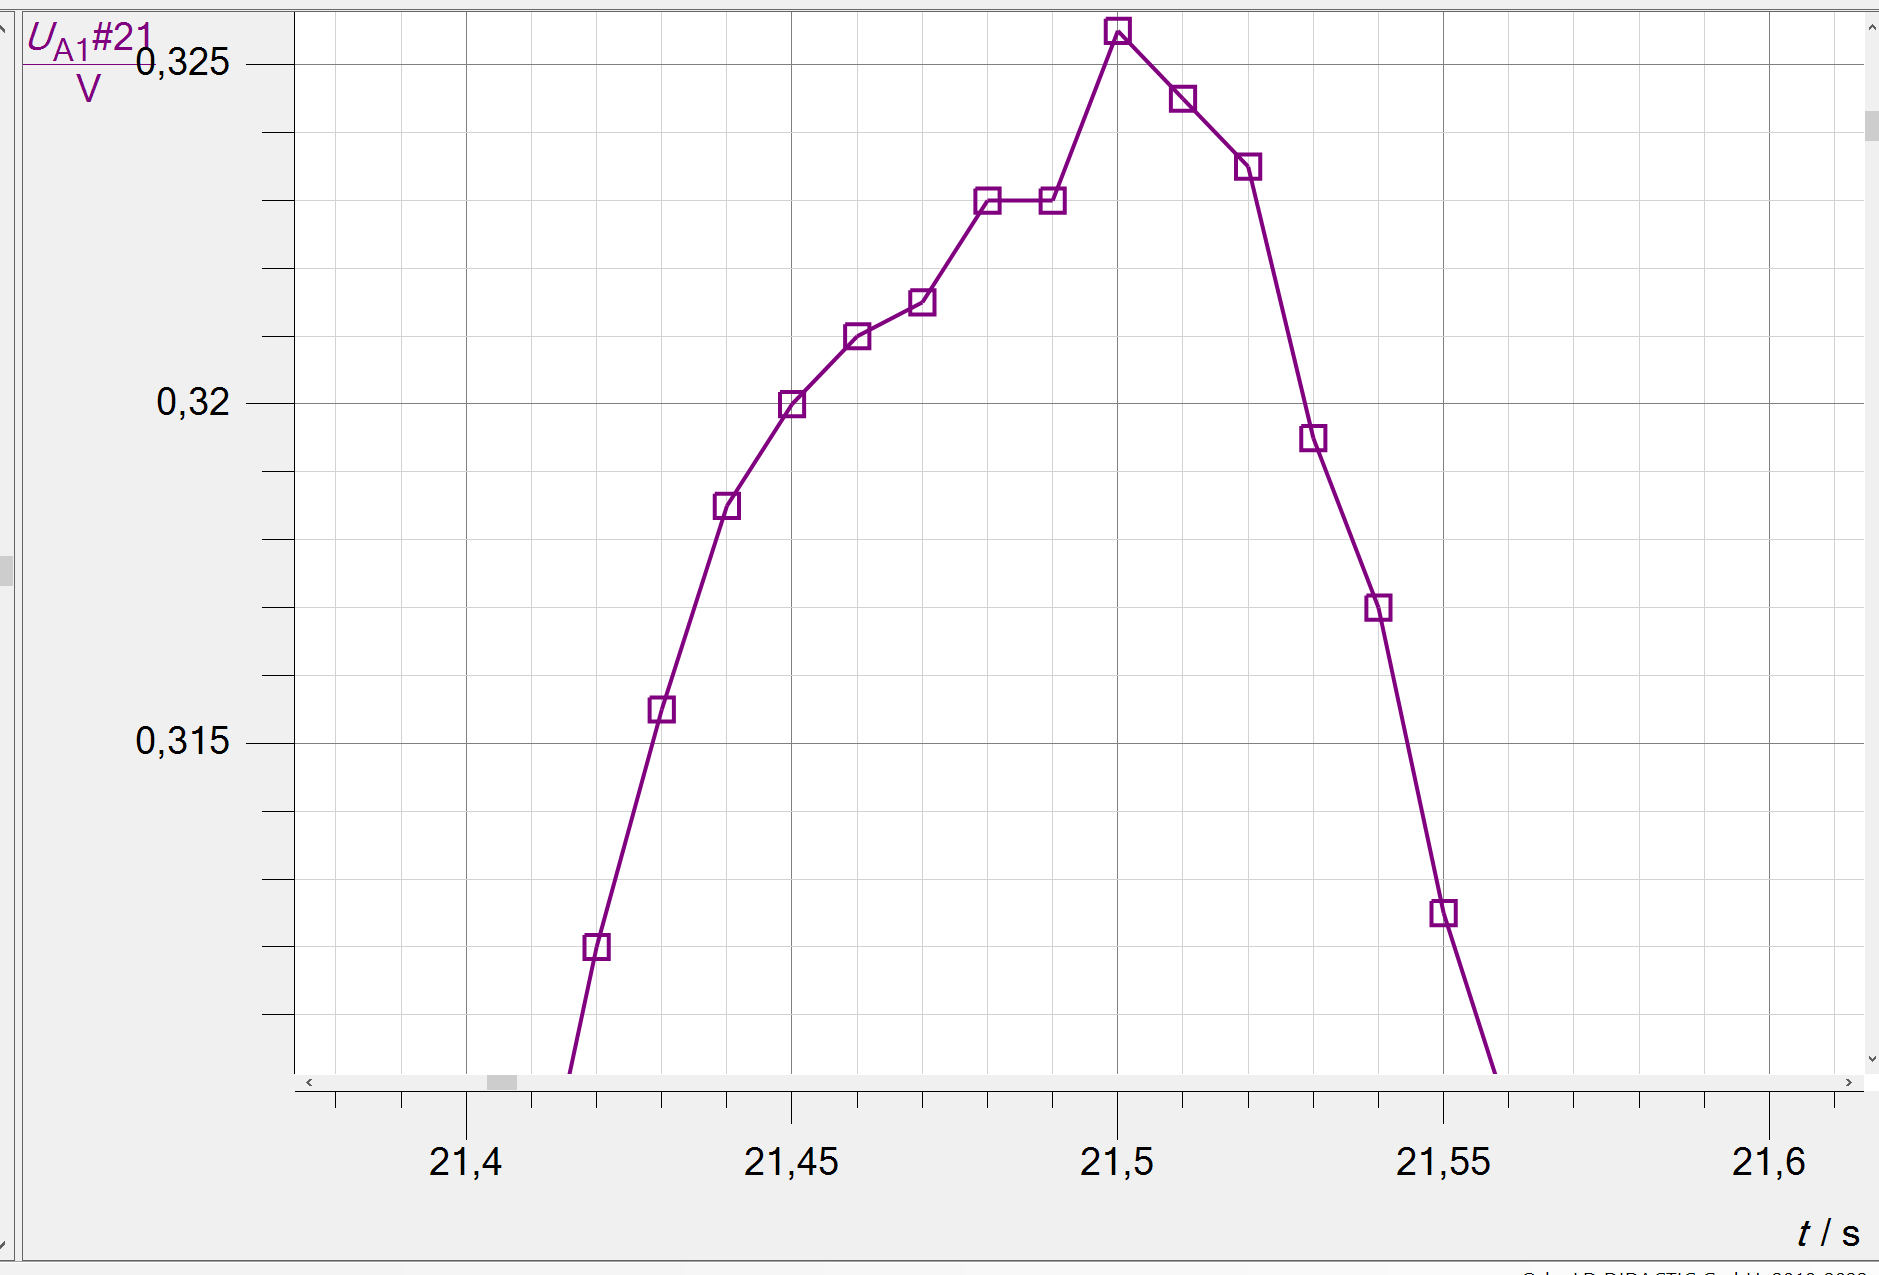
\includegraphics[width=0.6\textwidth]{plots/gewicht-2-peak.PNG}
    \caption{Peak der zweiten Messung mit Pendelkörper}
    \end{figure}
     
     
\begin{aufgabe}{Auswertung}
  Bestimmen Sie für alle Messreihen die Periodendauer und ihre
  Messunsicherheit, indem Sie eine geeignete lineare Regression
  durchführen. Demonstrieren Sie, dass Sie das Trägheitsmoment der
  Stange kompensiert haben. Tabellieren Sie die Zwischenergebnisse
  der relevanten Größen samt ihrer Messunsicherheiten. Berechnen
  Sie die Erdbeschleunigung. Führen Sie eine Fehlerrechnung zur
  Bestimmung der Messunsicherheit durch. Geben Sie bei Ihrer
  Fehlerrechnung die Größe der Einzelbeiträge an, die zu dem
  Gesamtfehler führen. Diskutieren Sie, welcher Fehler den
  Gesamtfehler dominiert. Vergleichen Sie Ihr Endergebnis mit dem
  relevanten Literaturwert.
\end{aufgabe}

\end{document}


%TODO : g neu berechnen auf Protokoll
%TODO : Auf messprotokoll noch das ablesen genauer drauf schreiben und now für letzten zwei messungen überschlag hinzufügen aber in falsch
 
 
